\chapter{Trouver des choses importantes/intéressantes dans le code}

Le minimalisme n'est pas une caractéristique prépondérante des logiciels modernes.

\myindex{\Cpp!STL}

Pas parce que les programmeurs écrivent beaucoup, mais parce que de nombreuses bibliothèques
sont couramment liées statiquement aux fichiers exécutable.
Si toutes les bibliothèques externes étaient déplacées dans des fichiers DLL externes,
le monde serait différent. (Une autre raison pour C++ sont la \ac{STL} et autres
bibliothèques templates.)

\newcommand{\FOOTNOTEBOOST}{\footnote{\url{http://www.boost.org/}}}
\newcommand{\FOOTNOTELIBPNG}{\footnote{\url{http://www.libpng.org/pub/png/libpng.html}}}

Ainsi, il est très important de déterminer l'origine de la fonction, si elle provient
d'une bibliothèque standard ou d'une bibliothèque bien connue (comme Boost\FOOTNOTEBOOST,
libpng\FOOTNOTELIBPNG), ou si elle est liée à ce que l'on essaye de trouver dans
le code.

Il est simplement absurde de tout récrire le code en \CCpp pour trouver ce que l'on
cherche.

Une des premières tâches d'un rétro-ingénieur est de trouver rapidement le code dont
il a besoin.

\myindex{\GrepUsage}

Le dés-assembleur \IDA nous permet de chercher parmi les chaînes de texte, les séquences
d'octets et les constantes.
Il est même possible d'exporter le code dans un fichier texte .lst ou .asm et d'utiliser
\TT{grep}, \TT{awk}, etc.

Lorsque vous essayez de comprendre ce que fait un certain code, ceci peut être facile
avec une bibliothèque open-source comme libpng.
Donc, lorsque vous voyez certaines constantes ou chaînes de texte qui vous semblent
familières, il vaut toujours la peine de les \emph{googler}.
Et si vous trouvez le projet open-source où elles sont utilisées, alors il suffit
de comparer les fonctions.
Ceci peut permettre de résoudre certaines parties du problème.

Par exemple, si un programme utilise des fichiers XML, la premières étape peut-être
de déterminer quelle bibliothèque XML est utilisée pour le traitement, puisque les
bibliothèques standards (ou bien connues) sont en général utilisées au lieu de code
fait maison.

\myindex{SAP}
\myindex{Windows!PDB}

Par exemple, j'ai essayé une fois de comprendre comment la compression/décompression
des paquets réseau fonctionne dans SAP 6.0.
C'est un logiciel gigantesque, mais un .\gls{PDB} détaillé avec des informations
de débogage est présent, et c'est pratique.
J'en suis finalement arrivé à l'idée que l'une des fonctions, qui était appelée par
\emph{CsDecomprLZC}, effectuait la décompression des paquets réseau.
Immédiatement, j'ai essayé de googler le nom et rapidement trouvé que la fonction
était utilisée dans MaxDB (c'est un projet open-source de SAP)
\footnote{Plus sur ce sujet dans la section concernée~(\myref{sec:SAPGUI})}.

\url{http://www.google.com/search?q=CsDecomprLZC}

Étonnement, les logiciels MaxDB et SAP 6.0 partagent du code comme ceci pour la compression/
décompression des paquets réseau.

\mysection{Identification de fichiers exécutables}

\subsection{Microsoft Visual C++}
\label{MSVC_versions}

Les versions de MSVC et des DLLs peuvent être importées:

%\small
\begin{center}
\begin{tabular}{ | l | l | l | l | l | }
\hline
\HeaderColor Marketing ver. &
\HeaderColor Internal ver. &
\HeaderColor CL.EXE ver. &
\HeaderColor DLLs imported &
\HeaderColor Release date \\
\hline
% 4.0, April 1995
% 97 & 5.0 & February 1997
6		&  6.0	& 12.00	& msvcrt.dll	& June 1998		\\
		&	&	& msvcp60.dll	&			\\
\hline
.NET (2002)	&  7.0	& 13.00	& msvcr70.dll	& February 13, 2002	\\
		&	&	& msvcp70.dll	&			\\
\hline
.NET 2003	&  7.1	& 13.10 & msvcr71.dll	& April 24, 2003	\\
		&	&	& msvcp71.dll	&			\\
\hline
2005		&  8.0	& 14.00 & msvcr80.dll	& November 7, 2005	\\
		&	&	& msvcp80.dll	&			\\
\hline
2008		&  9.0	& 15.00 & msvcr90.dll	& November 19, 2007	\\
		&	&	& msvcp90.dll	&			\\
\hline
2010		& 10.0	& 16.00 & msvcr100.dll	& April 12, 2010 	\\
		&	&	& msvcp100.dll	&			\\
\hline
2012		& 11.0	& 17.00 & msvcr110.dll	& September 12, 2012 	\\
		&	&	& msvcp110.dll	&			\\
\hline
2013		& 12.0	& 18.00 & msvcr120.dll	& October 17, 2013 	\\
		&	&	& msvcp120.dll	&			\\
\hline
\end{tabular}
\end{center}
%\normalsize

msvcp*.dll contient des fonctions relatives à \Cpp{}, donc si elle est importées,
il s'agit probablement d'un programme \Cpp.

\subsubsection{Mangling de nom}

Les noms commencent en général par le symbole \TT{?}.

Vous trouverez plus d'informations le \glslink{name mangling}{mangling de nom} de
MSVC ici: \myref{namemangling}.

\subsection{GCC}
\myindex{GCC}

À part les cibles *NIX, GCC est aussi présent dans l'environnement win32, sous la
forme de Cygwin et MinGW.

\subsubsection{Mangling de nom}

Les noms commencent en général par le symbole \TT{\_Z}.
Vous trouverez plus d'informations le \glslink{name mangling}{mangling de nom} de
GCC ici: \myref{namemangling}.
\subsubsection{Cygwin}
\myindex{Cygwin}

cygwin1.dll est souvent importée.

\subsubsection{MinGW}
\myindex{MinGW}

msvcrt.dll peut être importée.

\subsection{Intel Fortran}
\myindex{Fortran}

libifcoremd.dll, libifportmd.dll et libiomp5md.dll (support OpenMP) peuvent être importées.

libifcoremd.dll a beaucoup de fonctions préfixées par \TT{for\_}, qui signifie \emph{Fortran}.

\subsection{Watcom, OpenWatcom}
\myindex{Watcom}
\myindex{OpenWatcom}

\subsubsection{Mangling de nom}

Les noms commencent usuellement par le symbole \TT{W}.

Par exemple, ceci est la façon dont la méthode nommées \q{method} de la classe \q{class}
qui n'a pas d'argument et qui renvoie \Tvoid est encodée:

\begin{lstlisting}
W?method$_class$n__v
\end{lstlisting}

\subsection{Borland}
\myindex{Borland Delphi}
\myindex{Borland C++Builder}

Voici un exemple de \glslink{name mangling}{mangling de nom} de Delphi de Borland
et de C++Builder:

\lstinputlisting{digging_into_code/identification/borland_mangling.txt}

Les noms commencent toujours avec le symbole \TT{@}, puis nous avons le nom de la
classe, de la méthode et les types des arguments de méthode encodés.

Ces noms peuvent être dans des imports .exe, des exports .dll, des données de débogage,
etc.

Les Borland Visual Component Libraries (VCL) sont stockées dans des fichiers .bpl
au lieu de .dll, par exemple, vcl50.dll, rtl60.dll.

Une autre DLL qui peut être importée: BORLNDMM.DLL.

\subsubsection{Delphi}

Presque tous les exécutables Delpi ont la chaîne de texte \q{Boolean} au début de
leur segment de code, ainsi que d'autres noms de type.

Ceci est le début très typique du segment \TT{CODE} d'un programme Delphi, ce bloc
vient juste après l'entête de fichier win32 PE:

\lstinputlisting{digging_into_code/identification/delphi.txt}

Les 4 premiers octets du segment de données (\TT{DATA}) peuvent être \TT{00 00 00 00},
\TT{32 13 8B C0} ou \TT{FF FF FF FF}.%

Cette information peut être utile lorsque l'on fait face à des exécutables Delphi
préparés/chiffrés.

\subsection{Autres DLLs connues}

\myindex{OpenMP}
\begin{itemize}
\item vcomp*.dll---implémentation d'OpenMP de Microsoft.
\end{itemize}


% binary files might be also here

\mysection{Communication avec le monde extérieur (niveau fonction)}
Il est souvent recommandé de suivre les arguments de la fonction et sa valeur de
retour dans un débogueur ou \ac{DBI}.
Par exemple, l'auteur a essayé une fois de comprendre la signification d'une fonction
obscure, qui s'est avérée être un tri à bulles mal implémenté\footnote{\url{https://yurichev.com/blog/weird_sort_KLEE/}}.
(Il fonctionnait correctement, mais plus lentement.)
En même temps, regarder les entrées et sorties de cette fonction aide instantanément
à comprendre ce quelle fait.

Souvent, lorsque vous voyez une division par la multiplication (\myref{sec:divisionbymult}),
mais avez oublié tous les détails du mécanisme, vous pouvez seulement observer l'entrée
et la sortie, et trouver le diviseur rapidement.

% sections:
\mysection{Communication avec le monde extérieur (win32)}

Parfois, il est suffisant d'observer les entrées/sorties d'une fonction pour comprendre
ce qu'elle fait.
Ainsi, vous pouvez gagner du temps.

Accès aux fichiers et au registre:
pour les analyses très basiques, l'utilitaire, Process Monitor\footnote{\url{http://technet.microsoft.com/en-us/sysinternals/bb896645.aspx}}
de SysInternals peut aider.

Pour l'analyse basique des accès au réseau, Wireshark\footnote{\url{http://www.wireshark.org/}}
peut être utile.

Mais vous devrez de toutes façons regarder à l'intérieur, \\
\\
Les premières choses à chercher sont les fonctions des \ac{API}s de l'\ac{OS} et
des bibliothèques standards qui sont utilisées.

Si le programme est divisé en un fichier exécutable et un groupe de fichiers DLL,
parfois le nom des fonctions dans ces DLLs peut aider.

Si nous sommes intéressés par exactement ce qui peut conduire à appeler \TT{MessageBox()}
avec un texte spécifique, nous pouvons essayer de trouver ce texte dans le segment
de données, trouver sa référence et trouver les points depuis lesquels le contrôle
peut être passé à l'appel à \TT{MessageBox()} qui nous intéresse.

\myindex{\CStandardLibrary!rand()}
Si nous parlons d'un jeu vidéo et que nous sommes intéressés par les évènements qui
y sont plus ou moins aléatoires, nous pouvons essayer de trouver la fonction \rand
ou sa remplaçante (comme l'algorithme du twister de Mersenne) et trouver les points
depuis lesquels ces fonctions sont appelées, et plus important, comment les résultats
sont utilisés.
% BUG in varioref: http://tex.stackexchange.com/questions/104261/varioref-vref-or-vpageref-at-page-boundary-may-loop
Un exemple: \myref{chap:color_lines}.

Mais si ce n'est pas un jeu, et que \rand est toujours utilisé, il est intéressant
de savoir pourquoi.
Il a y des cas d'utilisation inattendu de \rand dans des algorithmes de compression
de données (pour une imitation du chiffrement):
\href{http://blog.yurichev.com/node/44}{blog.yurichev.com}.

\subsection{Fonctions souvent utilisées dans l'API Windows}

Ces fonctions peuvent être parmi les fonctions importées.
Il est utile de noter que toutes les fonctions ne sont pas forcément utilisées dans
du code écrit par le programmeur.
Beaucoup de fonctions peuvent être appelées depuis des fonctions de bibliothèque
et du code \ac{CRT}.

Certaines fonctions peuvent avoir le suffixe \GTT{-A} pour la version ASCII et \GTT{-W}
pour la version Unicode.

\begin{itemize}

\item
Accès au registre (advapi32.dll): 
RegEnumKeyEx, RegEnumValue, RegGetValue, RegOpenKeyEx, RegQueryValueEx.

\item
Accès au text des fichiers .ini (kernel32.dll):
GetPrivateProfileString.

\item
Boites de dialogue (user32.dll):
MessageBox, MessageBoxEx, CreateDialog, SetDlgItemText, GetDlgItemText.

\item
Accès aux resources (\myref{PEresources}): (user32.dll): LoadMenu.

\item
Réseau TCP/IP (ws2\_32.dll):
WSARecv, WSASend.

\item
Accès fichier (kernel32.dll):
CreateFile, ReadFile, ReadFileEx, WriteFile, WriteFileEx.

\item
Accès haut niveau à Internet (wininet.dll):
WinHttpOpen.

\item
Vérifier la signature digitale d'uin fichier exécutable (wintrust.dll):
WinVerifyTrust.

\item
La bibliothèque MSVC standard (si elle est liée dynamiquement) (msvcr*.dll):
assert, itoa, ltoa, open, printf, read, strcmp, atol, atoi, fopen, fread, fwrite, memcmp, rand,
strlen, strstr, strchr.

\end{itemize}

\subsection{Étendre la période d'essai}

Les fonctions d'accès au registre sont des cibles fréquentes pour ceux qui veulent
essayer de craquer des logiciels avec période d'essai, qui peuvent sauvegarder la
date et l'heure dans un registre.

Des autres cibles courantes sont les fonctions GetLocalTime() et GetSystemTime():
un logiciel avec période d'essai, à chaque démarrage, doit de toutes façons vérifier
la date et l'heure d'une certaine façon.

\subsection{Supprimer la boite de dialogue nag}

Une manière répandue de trouver ce qui cause l'apparition de la boite de dialogue
nag est d'intercepter les fonctions MessageBox(), CreateDialog() et CreateWindow().

\subsection{tracer: Intercepter toutes les fonctions dans un module spécifique}
\myindex{tracer}

\myindex{x86!\Instructions!INT3}
Il y a un point d'arrêt INT3 dans \tracer, qui peut être déclenché seulement une
fois, toutefois, il peut être mis pour toutes les fonctions dans une DLL spécifique.

\begin{lstlisting}
--one-time-INT3-bp:somedll.dll!.*
\end{lstlisting}

Ou, mettons un point d'arrêt INT3 sur toutes les fonctions avec le préfixe \TT{xml}
dans leur nom:

\begin{lstlisting}
--one-time-INT3-bp:somedll.dll!xml.*
\end{lstlisting}

Le revers de la médaille est que de tels points d'arrêt ne sont déclenchés qu'une fois.
Tracer montrera l'appel à une fonction, s'il se produit, mais seulement une fois.
Un autre inconvénient---il est impossible de voir les arguments de la fonction.

Néanmoins, cette fonctionnalité est très utile lorsque vous avez qu'un programme
utilise une DLL, mais que vous ne savez pas quelles fonctions sont effectivement
utilisées.
Et il y a beaucoup de fonctions.

\par
\myindex{Cygwin}
Par exemple, regardons ce qu'utilise l'utilitaire uptime de Cygwin:

\begin{lstlisting}
tracer -l:uptime.exe --one-time-INT3-bp:cygwin1.dll!.*
\end{lstlisting}

Ainsi nous pouvons voir quelles sont les fonctions de la bibliothèque cygwin1.dll
qui sont appelées au moins une fois, et depuis où:

\lstinputlisting{digging_into_code/uptime_cygwin.txt}


\mysection{Chaînes}
\label{sec:digging_strings}

\subsection{Exemple \#2: SCO OpenServer}

\label{examples_SCO}
\myindex{SCO OpenServer}
Un ancien logiciel pour SCO OpenServer de 1997 développé par une société qui a disparue
depuis longtemps.

Il y a un driver de dongle special à installer dans le système, qui contient les
chaînes de texte suivantes:
\q{Copyright 1989, Rainbow Technologies, Inc., Irvine, CA}
et
\q{Sentinel Integrated Driver Ver. 3.0 }.

Après l'installation du driver dans SCO OpenServer, ces fichiers apparaissent dans
l'arborescence /dev:

\begin{lstlisting}
/dev/rbsl8
/dev/rbsl9
/dev/rbsl10
\end{lstlisting}

Le programme renvoie une erreur lorsque le dongle n'est pas connecté, mais le message
d'erreur n'est pas trouvé dans les exécutables.

\myindex{COFF}

Grâce à \ac{IDA}, il est facile de charger l'exécutable COFF utilisé dans SCO OpenServer.

Essayons de trouver la chaîne \q{rbsl} et en effet, elle se trouve dans ce morceau
de code:

\lstinputlisting[style=customasmx86]{examples/dongles/2/1.lst}

Oui, en effet, le programme doit communiquer d'une façon ou d'une autre avec le driver.

\myindex{thunk-functions}
Le seul endroit où la fonction \TT{SSQC()} est appelée est dans la \glslink{thunk
 function}{fonction thunk}:

\lstinputlisting[style=customasmx86]{examples/dongles/2/2.lst}

SSQ() peut être appelé depuis au moins 2 fonctions.

L'une d'entre elles est:

\lstinputlisting[style=customasmx86]{examples/dongles/2/check1_EN.lst}

\q{\TT{3C}} et \q{\TT{3E}} semblent familiers: il y avait un dongle Sentinel Pro de
Rainbow sans mémoire, fournissant seulement une fonction de crypto-hachage secrète.

Vous pouvez lire une courte description de la fonction de hachage dont il s'agit
ici: \myref{hash_func}.

Mais retournons au programme.

Donc le programme peut seulement tester si un dongle est connecté ou s'il est absent.

Aucune autre information ne peut être écrite dans un tel dongle, puisqu'il n'a pas
de mémoire.
Les codes sur deux caractères sont des commandes (nous pouvons voir comment les commandes
sont traitées dans la fonction \TT{SSQC()}) et toutes les autres chaînes sont hachées
dans le dongle, transformées en un nombre 16-bit.
L'algorithme était secret, donc il n'était pas possible d'écrire un driver de remplacement
ou de refaire un dongle matériel qui l'émulerait parfaitement.

Toutefois, il est toujours possible d'intercepter tous les accès au dongle et de
trouver les constantes auxquelles les résultats de la fonction de hachage sont comparées.

Mais nous devons dire qu'il est possible de construire un schéma de logiciel de protection
de copie robuste basé sur une fonction secrète de hachage cryptographique: il suffit
qu'elle chiffre/déchiffre les fichiers de données utilisés par votre logiciel.

Mais retournons au code:

Les codes 51/52/53 sont utilisés pour choisir le port imprimante LPT.
3x/4x sont utilisés pour le choix de la \q{famille} (c'est ainsi que les dongles
Sentinel Pro sont différenciés les uns des autres: plus d'un dongle peut être connecté
sur un port LPT).

La seule chaîne passée à la fonction qui ne fasse pas 2 caractères est "0123456789".

Ensuite, le résultat est comparé à l'ensemble des résultats valides.

Si il est correct, 0xC ou 0xB est écrit dans la variable globale \TT{ctl\_model}.%

Une autre chaîne de texte qui est passée est
"PRESS ANY KEY TO CONTINUE: ", mais le résultat n'est pas testé.
Difficile de dire pourquoi, probablement une erreur\footnote{C'est un sentiment
étrange de trouver un bug dans un logiciel aussi ancien.}.

Voyons où la valeur de la variable globale \TT{ctl\_model} est utilisée.

Un tel endroit est:

\lstinputlisting[style=customasmx86]{examples/dongles/2/4.lst}

Si c'est 0, un message d'erreur chiffré est passé à une routine de déchiffrement
et affiché.

\myindex{x86!\Instructions!XOR}

La routine de déchiffrement de la chaîne semble être un simple \glslink{xoring}{xor}:

\lstinputlisting[style=customasmx86]{examples/dongles/2/err_warn.lst}

C'est pourquoi nous étions incapable de trouver le message d'erreur dans les fichiers
exécutable, car ils sont chiffrés (ce qui est une pratique courante).

Un autre appel à la fonction de hachage \TT{SSQ()} lui passe la chaîne \q{offln}
et le résultat est comparé avec \TT{0xFE81} et \TT{0x12A9}.

Si ils ne correspondent pas, ça se comporte comme une sorte de fonction \TT{timer()}
(peut-être en attente qu'un dongle mal connecté soit reconnecté et re-testé?) et ensuite
déchiffre un autre message d'erreur à afficher.

\lstinputlisting[style=customasmx86]{examples/dongles/2/check2_EN.lst}

Passer outre le dongle est assez facile: il suffit de patcher tous les sauts après
les instructions \CMP pertinentes.

Une autre option est d'écrire notre propre driver SCO OpenServer, contenant une table
de questions et de réponses, toutes celles qui sont présentent dans le programme.

\subsubsection{Déchiffrer les messages d'erreur}

À propos, nous pouvons aussi essayer de déchiffrer tous les messages d'erreurs.
L'algorithme qui se trouve dans la fonction \TT{err\_warn()} est très simple, en effet:

\lstinputlisting[caption=Decryption function,style=customasmx86]{examples/dongles/2/decrypting_FR.lst}

Comme on le voit, non seulement la chaîne est transmise à la fonction de déchiffrement
mais aussi la clef:

\lstinputlisting[style=customasmx86]{examples/dongles/2/tmp1_EN.asm}

L'algorithme est un simple \glslink{xoring}{xor}: chaque octet est xoré avec la clef, mais
la clef est incrémentée de 3 après le traitement de chaque octet.

Nous pouvons écrire un petit script Python pour vérifier notre hypothèse:

\lstinputlisting[caption=Python 3.x]{examples/dongles/2/decr1.py}

Et il affiche: \q{check security device connection}.
Donc oui, ceci est le message déchiffré.

Il y a d'autres messages chiffrés, avec leur clef correspondante.
Mais inutile de dire qu'il est possible de les déchiffrer sans leur clef.
Premièrement, nous voyons que le clef est en fait un octet.
C'est parce que l'instruction principale de déchiffrement (\XOR) fonctionne au niveau
de l'octet.
La clef se trouve dans le registre \ESI, mais seulement une partie de \ESI d'un octet
est utilisée.
Ainsi, une clef pourrait être plus grande que 255, mais sa valeur est toujours arrondie.

En conséquence, nous pouvons simplement essayer de brute-forcer, en essayant toutes
les clefs possible dans l'intervalle 0..255.
Nous allons aussi écarter les messages comportants des caractères non-imprimable.

\lstinputlisting[caption=Python 3.x]{examples/dongles/2/decr2.py}

Et nous obtenons:

\lstinputlisting[caption=Results]{examples/dongles/2/decr2_result.txt}

Ici il y a un peu de déchet, mais nous pouvons rapidement trouver les messages en
anglais.

À propos, puisque l'algorithme est un simple chiffrement xor, la même fonction peut
être utilisée pour chiffrer les messages.
Si besoin, nous pouvons chiffrer nos propres messages, et patcher le programme en les insérant.


\subsection{Trouver des chaînes dans un binaire}

\epigraph{Actually, the best form of Unix documentation is frequently running the
\textbf{strings} command over a program’s object code. Using \textbf{strings}, you can get
a complete list of the program’s hard-coded file name, environment variables,
undocumented options, obscure error messages, and so forth.}{The Unix-Haters Handbook}
En fait, la meilleure forme de documentation Unix est de lancer la commande
\textbf{strings} sur le code objet d'un programme. En utilisant \textbf{strings},
vous obtenez une liste complète des noms de fichiers codés en dur dans le programme,
les variables d'environnement, les options non documentées, les messages d'erreurs
méconnus et ainsi de suite.

\myindex{UNIX!strings}
L'utilitaire standard UNIX \emph{strings} est un moyen rapide et facile de voir les
chaînes dans un fichier.
Par exemple, voici quelques chaînes du fichier exécutable sshd d'OpenSSH 7.2:

\lstinputlisting{digging_into_code/sshd_strings.txt}

Il y a des options, des messages d'erreur, des chemins de fichier, des modules et
des fonctions importés dynamiquement, ainsi que d'autres chaînes étranges (clefs?).
Il y a aussi du bruit illisible---le code x86 à parfois des fragments constitués de
caractères ASCII imprimables, jusqu'à ~8 caractères.

Bien sûr, OpenSSH est un programme open-source.
Mais regarder les chaînes lisibles dans un binaire inconnu est souvent une première
étape d'analyse.
\myindex{UNIX!grep}

\emph{grep} peut aussi être utilisé.

\myindex{Hiew}
\myindex{Sysinternals}
Hiew a la même capacité (Alt-F6), ainsi que ProcessMonitor de Sysinternals.

\subsection{Messages d'erreur/de débogage}

Les messages de débogage sont très utiles s'il sont présents.
Dans un certain sens, les messages de débogage rapportent ce qui est en train de
se passer dans le programme. Souvent, ce sont des fonctions \printf-like, qui écrivent
des fichiers de log, ou parfois elles n'écrivent rien du tout mais les appels sont
toujours présents puisque le build n'est pas un de débogage mais de \emph{release}.
\myindex{\oracle}

Si des variables locales ou globales sont affichées dans les messages, ça peut être
aussi utile, puisqu'il est possible d'obtenir au moins le nom de la variable.
Par exemple, une telle fonction dans \oracle est \TT{ksdwrt()}.

Des chaînes de texte significatives sont souvent utiles.
Le dés-assembleur \IDA peut montrer depuis quelles fonctions et depuis quel endroit
cette chaîne particulière est utilisée.
Des cas drôles arrivent parfois\footnote{\href{http://blog.yurichev.com/node/32}{blog.yurichev.com}}.

Le message d'erreur peut aussi nous aider.
Dans \oracle, les erreurs sont rapportées en utilisant un groupe de fonctions.\\
Vous pouvez en lire plus ici: \href{http://blog.yurichev.com/node/43}{blog.yurichev.com}.

\myindex{Error messages}

Il est possible de trouver rapidement quelle fonction signale une erreur et dans
quelles conditions.

À propos, ceci est souvent la raison pour laquelle les systèmes de protection contre
la copie utilisent des messages d'erreur inintelligibles ou juste des numéros d'erreur.
Personne n'est content lorsque le copieur de logiciel comprend comment fonctionne
la protection contre la copie seulement en lisant les messages d'erreur.

Un exemple de messages d'erreur chiffrés se trouve ici: \myref{examples_SCO}.

\subsection{Chaînes magiques suspectes}

Certaines chaînes magique sont d'habitude utilisées dans les porte dérobées semblent
vraiment suspectes.

Par exemple, il y avait une porte dérobée dans le routeur personnel TP-Link WR740%
\footnote{\url{http://sekurak.pl/tp-link-httptftp-backdoor/}}.
La porte dérobée était activée en utilisant l'URL suivante:\\
\url{http://192.168.0.1/userRpmNatDebugRpm26525557/start_art.html}.\\

En effet, la chaîne \q{userRpmNatDebugRpm26525557} est présente dans le firmware.

Cette chaîne n'était pas googlable jusqu'à la large révélation d'information concernant
la porte dérobée.

Vous ne trouverez ceci dans aucun \ac{RFC}.

Vous ne trouverez pas d'algorithme informatique qui utilise une séquence d'octets
aussi étrange.

Et elle ne ressemble pas à une erreur ou un message de débogage.

Donc, c'est une bonne idée d'inspecter l'utilisation de ce genre de chaînes bizarres.\\
\\
\myindex{base64}

Parfois, de telles chaînes sont encodées en utilisant base64.

Donc, c'est une bonne idée de toutes les décoder et de les inspecter visuellement,
même un coup d'\oe{}il doit suffire.\\
\\
\myindex{Sécurité par l'obscurité}
Plus précisément, cette méthode de cacher des accès non documentés est appelée \q{sécurité par l'obscurité}.


\mysection{Appels à assert()}
\myindex{\CStandardLibrary!assert()}

Parfois, la présence de la macro \TT{assert()} est aussi utile:
En général, cette macro laisse le nom du fichier source, le numéro de ligne et une
condition dans le code.

L'information la plus utile est contenue dans la condition d'assert, nous pouvons
en déduire les noms de variables ou les noms de champ de la structure. Les autres
informations utiles sont les noms de fichier---nous pouvons essayer d'en déduire
le type de code dont il s'agit ici.
Il est aussi possible de reconnaître les bibliothèques open-source connues d'après
les noms de fichier.

\lstinputlisting[caption=Exemple d'appels à assert() informatifs,style=customasmx86]{digging_into_code/assert_examples.lst}

Il est recommandé de \q{googler} à la fois les conditions et les noms de fichier,
qui peuvent nous conduire à une bibliothèque open-source.
Par exemple, si nous \q{googlons} \q{sp->lzw\_nbits <= BITS\_MAX}, cela va comme
prévu nous donner du code open-source relatif à la compression LZW.

\mysection{Constantes}

Les humains, programmeurs inclus, utilisent souvent des nombres ronds, comme 10, 100,
1000, dans la vie courante comme dans le code.

Le rétro ingénieur pratiquant connaît en général bien leur représentation décimale:
10=0xA, 100=0x64, 1000=0x3E8, 10000=0x2710.

Les constantes \TT{0xAAAAAAAA} (0b10101010101010101010101010101010) et \\
\TT{0x55555555} (0b01010101010101010101010101010101)  sont aussi répandues---elles
sont composées d'alternance de bits.

Cela peut aider à distinguer un signal d'un signal dans lequel tous les bits sont
à 1 (0b1111 \dots) ou à 0 (0b0000 \dots).
Par exemple, la constante \TT{0x55AA} est utilisée au moins dans le secteur de boot,
\ac{MBR}, et dans la \ac{ROM} de cartes d'extention de compatible IBM.

Certains algorithmes, particulièrement ceux de chiffrement, utilisent des constantes
distinctes, qui sont faciles à trouver dans le code en utilisant \IDA.

\myindex{MD5}

Par exemple, l'algorithme MD5 initialise ses propres
variables internes comme ceci:

\begin{verbatim}
var int h0 := 0x67452301
var int h1 := 0xEFCDAB89
var int h2 := 0x98BADCFE
var int h3 := 0x10325476
\end{verbatim}

Si vous trouvez ces quatre constantes utilisées à la suite dans du code, il est
très probable que cette fonction soit relatives à MD5.

\par Un autre exemple sont les algorithmes CRC16/CRC32, ces algorithmes de calcul
utilisent souvent des tables pré-calculées comme celle-ci:

\begin{lstlisting}[caption=linux/lib/crc16.c,style=customc]
/** CRC table for the CRC-16. The poly is 0x8005 (x^16 + x^15 + x^2 + 1) */
u16 const crc16_table[256] = {
	0x0000, 0xC0C1, 0xC181, 0x0140, 0xC301, 0x03C0, 0x0280, 0xC241,
	0xC601, 0x06C0, 0x0780, 0xC741, 0x0500, 0xC5C1, 0xC481, 0x0440,
	0xCC01, 0x0CC0, 0x0D80, 0xCD41, 0x0F00, 0xCFC1, 0xCE81, 0x0E40,
	...
\end{lstlisting}

Voir aussi la table pré-calculée pour CRC32: \myref{sec:CRC32}.

Dans les algorithmes CRC sans table, des polynômes bien connus sont utilisés, par
exemple 0xEDB88320 pour CRC32.

\subsection{Nombres magiques}
\label{magic_numbers}

De nombreux formats de fichier définissent un entête standard où un \emph{nombre(s) magique}
est utilisé, unique ou même plusieurs.

\myindex{MS-DOS}

Par exemple, tous les exécutables Win32 et MS-DOS débutent par ces deux caractères \q{MZ}\footnote{\href{http://en.wikipedia.org/wiki/DOS_MZ_executable}{Wikipédia}}.

\myindex{MIDI}

Au début d'un fichier MIDI, la signature \q{MThd} doit être présente.
Si nous avons un programme qui utilise des fichiers MIDI pour quelque chose, il
est très probable qu'il doit vérifier la validité du fichier en testant au moins
les 4 premiers octets.

Ça peut être fait comme ceci:
(\emph{buf} pointe sur le début du fichier chargé en mémoire)

\begin{lstlisting}[style=customasmx86]
cmp [buf], 0x6468544D ; "MThd"
jnz _error_not_a_MIDI_file
\end{lstlisting}

\myindex{\CStandardLibrary!memcmp()}
\myindex{x86!\Instructions!CMPSB}

\dots ou en appelant une fonction pour comparer des blocs de mémoire comme \TT{memcmp()}
ou tout autre code équivalent jusqu'à une instruction \TT{CMPSB} (\myref{REPE_CMPSx}).

Lorsque vous trouvez un tel point, vous pouvez déjà dire que le chargement du fichier
MIDI commence, ainsi, vous pouvez voir l'endroit où se trouve le buffer avec le contenu
du fichier MIDI, ce qui est utilisé dans le buffer et comment.

\subsubsection{Dates}

\myindex{UFS2}
\myindex{FreeBSD}
\myindex{HASP}

Souvent, on peut rencontrer des nombres comme \TT{0x19870116}, qui ressemble clairement
à une date (année 1987, 1er mois (janvier), 16ème jour).
Ça peut être la date de naissance de quelqu'un (un programmeur, une de ses relations,
un enfant), ou une autre date importante.
La date peut aussi être écrite dans l'ordre inverse, comme \TT{0x16011987}.
Les dates au format américain sont aussi courante, comme \TT{0x01161987}.

Un exemple célèbre est \TT{0x19540119} (nombre magique utilisé dans la structure
du super-bloc UFS2), qui est la date de naissance de Marshall Kirk McKusick, éminent
contributeur FreeBSD.

\myindex{Stuxnet}
Stuxnet utilise le nombre ``19790509'' (pas comme un nombre 32-bit, mais comme une
chaîne, toutefois), et ça a conduit à spéculer que le malware était relié à Israël%
\footnote{C'est la date d'exécution de Habib Elghanian, juif persan.}.

Aussi, des nombres comme ceux-ci sont très répandus dans dans le chiffrement niveau
amateur, par exemple, extrait de la \emph{fonction secrète} des entrailles du dongle
HASP3\footnote{\url{https://web.archive.org/web/20160311231616/http://www.woodmann.com/fravia/bayu3.htm}}:

\begin{lstlisting}[style=customc]
void xor_pwd(void)
{
	int i;

	pwd^=0x09071966;
	for(i=0;i<8;i++)
	{
		al_buf[i]= pwd & 7; pwd = pwd >> 3;
	}
};

void emulate_func2(unsigned short seed)
{
	int i, j;
	for(i=0;i<8;i++)
	{
		ch[i] = 0;

		for(j=0;j<8;j++)
		{
			seed *= 0x1989;
			seed += 5;
			ch[i] |= (tab[(seed>>9)&0x3f]) << (7-j);
		}
	}
}
\end{lstlisting}

\subsubsection{DHCP}

Ceci s'applique aussi aux protocoles réseaux.
Par exemple, les paquets réseau du protocole DHCP contiennent un soi-disant \emph{nombre
magique}: \TT{0x63538263}.
Tout code qui génère des paquets DHCP doit contenir quelque part cette constante
à insérer dans les paquets.
Si nous la trouvons dans du code, nous pouvons trouver ce qui s'y passe, et pas seulement ça.
Tout programme qui peut recevoir des paquet DHCP doit vérifier le \emph{cookie magique},
et le comparer à cette constante.

Par exemple, prenons le fichier dhcpcore.dll de Windows 7 x64 et cherchons cette constante.
Et nous la trouvons, deux fois:
Il semble que la constante soit utilisée dans deux fonctions avec des noms parlants\\
\TT{DhcpExtractOptionsForValidation()} et \TT{DhcpExtractFullOptions()}:

\begin{lstlisting}[caption=dhcpcore.dll (Windows 7 x64),style=customasmx86]
.rdata:000007FF6483CBE8 dword_7FF6483CBE8 dd 63538263h          ; DATA XREF: DhcpExtractOptionsForValidation+79
.rdata:000007FF6483CBEC dword_7FF6483CBEC dd 63538263h          ; DATA XREF: DhcpExtractFullOptions+97
\end{lstlisting}

Et ici sont les endroits où ces constantes sont accédées:

\begin{lstlisting}[caption=dhcpcore.dll (Windows 7 x64),style=customasmx86]
.text:000007FF6480875F  mov     eax, [rsi]
.text:000007FF64808761  cmp     eax, cs:dword_7FF6483CBE8
.text:000007FF64808767  jnz     loc_7FF64817179
\end{lstlisting}

Et:

\begin{lstlisting}[caption=dhcpcore.dll (Windows 7 x64),style=customasmx86]
.text:000007FF648082C7  mov     eax, [r12]
.text:000007FF648082CB  cmp     eax, cs:dword_7FF6483CBEC
.text:000007FF648082D1  jnz     loc_7FF648173AF
\end{lstlisting}

\subsection{Constantes spécifiques}

Parfois, il y a une constante spécifique pour un certain type de code.
Par exemple, je me suis plongé une fois dans du code, où le nombre 12 était rencontré
anormalement souvent.
La taille de nombreux tableaux était 12 ou un multiple de 12 (24, etc.).
Il s'est avéré que ce code prenait des fichiers audio de 12 canaux en entrée et les
traitait.

Et vice versa: par exemple, si un programme fonctionne avec des champs de texte qui
ont une longueur de 120 octets, il doit y avoir une constante 120 ou 119 quelque
part dans le code.
Si UTF-16 est utilisé, alors $2 \cdot 120$.
Si le code fonctionne avec des paquets réseau de taille fixe, c'est une bonne idée
de chercher cette constante dans le code.

C'est aussi vrai pour le chiffrement amateur (clefs de licence, etc.).
Si le bloc chiffré a une taille de $n$ octets, vous pouvez essayer de trouver des
occurrences de ce nombre à travers le code.
Aussi, si vous voyez un morceau de code qui est répété $n$ fois dans une boucle durant
l'exécution, ceci peut être une routine de chiffrement/déchiffrement.

\subsection{Chercher des constantes}

C'est facile dans \IDA: Alt-B or Alt-I.
\myindex{binary grep}
Et pour chercher une constante dans un grand nombre de fichiers, ou pour chercher
dans des fichiers non exécutables, il y a un petit utilitaire appelé \emph{binary grep}\footnote{\BGREPURL}.


\subsection{Instructions}
\label{sec:x86_instructions}

Les instructions marquées avec un (M) ne sont généralement pas générées par le compilateur:
si vous rencontrez l'une d'entre elles, il s'agit probablement de code assembleur
écrit à la main, ou de fonctions intrinsèques (\myref{sec:compiler_intrinsic}).

% TODO ? обратные инструкции

Seules les instructions les plus fréquemment utilisées sont listées ici.
Vous pouvez lire \myref{x86_manuals} pour une documentation complète.

Devez-vous connaître tous les opcodes des instructions par c\oe{}ur?
Non, seulement ceux qui sont utilisés pour patcher du code
(\myref{x86_patching}).
Tout le reste des opcodes n'a pas besoin d'être mémorisé.

\subsubsection{Préfixes}

\myindex{x86!\Prefixes!LOCK}
\myindex{x86!\Prefixes!REP}
\myindex{x86!\Prefixes!REPE/REPNE}
\begin{description}
\label{x86_lock}
\item[LOCK] force le CPU à faire un accès exclusif à la RAM dans un environnement multi-processeurs.
Par simplification, on peut dire que lorsqu'une instruction avec ce préfixe est exécutée,
tous les autres CPU dans un système multi-processeur sont stoppés.
Le plus souvent, c'est utilisé pour les sections critiques, les sémaphores et les mutex.
Couramment utilisé avec ADD, AND, BTR, BTS, CMPXCHG, OR, XADD, XOR.
Vous pouvez en lire plus sur les sections critiques ici (\myref{critical_sections}).

\item[REP] est utilisé avec les instructions MOVSx et STOSx:
exécute l'instruction dans une boucle, le compteur est situé dans le registre CX/ECX/RCX.
Pour une description plus détaillée de ces instructions, voir MOVSx (\myref{REP_MOVSx})
et STOSx (\myref{REP_STOSx}).

Les instructions préfixées par REP sont sensibles au flag DF, qui est utilisé pour définir la direction.

\item[REPE/REPNE] (\ac{AKA} REPZ/REPNZ) utilisé avec les instructions CMPSx et SCASx:
exécute la dernière instruction dans une boucle, le compteur est mis dans le registre \TT{CX}/\TT{ECX}/\TT{RCX}.
Elle s'arrête prématurément si ZF vaut 0 (REPE) ou si ZF vaut 1 (REPNE).

Pour une description plus détaillée de ces instructions, voir CMPSx (\myref{REPE_CMPSx})
et SCASx (\myref{REPNE_SCASx}).

Les instructions préfixées par REPE/REPNE sont sensibles au flag DF, qui est utilisé pour définir la direction.

\end{description}

\subsubsection{Instructions les plus fréquemment utilisées}

Celles-ci peuvent être mémorisées en premier.

\begin{description}
% in order to keep them easily sorted...
\myindex{x86!\Instructions!ADC}
\myindex{x86!\Flags!CF}
  \item[ADC] (\emph{add with carry})
  ajoute des valeurs, \glslink{increment}{incrémente} le résultat si le flag CF est
  mis. ADC est souvent utilisé pour ajouter des grandes valeurs, par exemple, pour
  ajouter deux valeurs 64-bit dans un environnement 32-bit en utilisant deux
  instructions, ADD et ADC. Par exemple:

\lstinputlisting[style=customasmx86]{appendix/x86/instructions/ADC_example_FR.lst}

Un autre exemple: \myref{sec:64bit_in_32_env}.

\myindex{x86!\Instructions!ADD}
  \item[ADD] \RU{сложить два значения}\EN{add two values}\FR{ajoute deux valeurs}

\myindex{x86!\Instructions!AND}
  \item[AND] \RU{логическое \q{И}}\EN{logical \q{and}}\FR{\q{et} logique}

\myindex{x86!\Instructions!CALL}
  \item[CALL] \RU{вызвать другую функцию}\EN{call another function}\FR{appelle une autre fonction}:\\
  \TT{PUSH address\_after\_CALL\_instruction; JMP label}

\myindex{x86!\Instructions!CMP}
\myindex{x86!\Instructions!SUB}
  \item[CMP] \RU{сравнение значений и установка флагов, то же что и \TT{SUB}, но только без записи результата}
  \EN{compare values and set flags, the same as \TT{SUB} but without writing the result}
  \FR{compare les valeurs et met les flags, comme \TT{SUB} mais sans écrire le résultat}

\myindex{x86!\Instructions!DEC}
\myindex{x86!\Flags!CF}
  \item[DEC] \glslink{decrement}{décrémente}.
Contrairement aux autres instructions arithmétiques, \TT{DEC} ne modifie pas
le flag CF.


\myindex{x86!\Instructions!IMUL}
  \item[IMUL] \RU{умножение с учетом знаковых значений}\EN{signed multiply}\FR{multiplication signée}
  \EN{\IMUL often used instead of \MUL, read more about it:}%
  \RU{\IMUL часто используется вместо \MUL, читайте об этом больше:}%
  \FR{\IMUL est souvent utilisé à la place de \MUL, voir ici:} \myref{IMUL_over_MUL}.


\myindex{x86!\Instructions!INC}
\myindex{x86!\Flags!CF}
  \item[INC] \glslink{increment}{incrémente}.
Contrairement aux autres instructions arithmétiques, \TT{INC} ne modifie pas
le flag CF.

\myindex{x86!\Instructions!JCXZ}
\myindex{x86!\Instructions!JECXZ}
\myindex{x86!\Instructions!JRCXZ}
  \item[JCXZ, JECXZ, JRCXZ] (M) \RU{переход если CX/ECX/RCX=0}\EN{jump if CX/ECX/RCX=0}\FR{saute si CX/ECX/RCX=0}

\myindex{x86!\Instructions!JMP}
\item[JMP] \RU{перейти на другой адрес}\EN{jump to another address}\FR{saute à une
autre adresse}.
\RU{Опкод имеет т.н.}\EN{The opcode has a}\FR{L'opcode a un} \gls{jump offset}.

\item[Jcc] (où cc ---  condition code)

\myindex{x86!\Instructions!JAE}
\myindex{x86!\Instructions!JA}
\myindex{x86!\Instructions!JBE}
\myindex{x86!\Instructions!JB}
\myindex{x86!\Instructions!JC}
\myindex{x86!\Instructions!JE}
\myindex{x86!\Instructions!JGE}
\myindex{x86!\Instructions!JG}
\myindex{x86!\Instructions!JLE}
\myindex{x86!\Instructions!JL}
\myindex{x86!\Instructions!JNAE}
\myindex{x86!\Instructions!JNA}
\myindex{x86!\Instructions!JNBE}
\myindex{x86!\Instructions!JNB}
\myindex{x86!\Instructions!JNC}
\myindex{x86!\Instructions!JNE}
\myindex{x86!\Instructions!JNGE}
\myindex{x86!\Instructions!JNG}
\myindex{x86!\Instructions!JNLE}
\myindex{x86!\Instructions!JNL}
\myindex{x86!\Instructions!JNO}
\myindex{x86!\Instructions!JNS}
\myindex{x86!\Instructions!JNZ}
\myindex{x86!\Instructions!JO}
\myindex{x86!\Instructions!JPO}
\myindex{x86!\Instructions!JP}
\myindex{x86!\Instructions!JS}
\myindex{x86!\Instructions!JZ}

Beaucoup de ces instructions ont des synonymes (notés avec AKA), qui ont été ajoutés
par commodité. Ils sont codés avec le même opcode.
L'opcode a un \glslink{jump offset}{offset de saut}.

\label{Jcc}
\begin{description}
\item[JAE] \ac{AKA} JNC: saut si supérieur ou égal (non signé): C=0
\item[JA] \ac{AKA} JNBE: saut si supérieur (non signé): CF=0 et ZF=0
\item[JBE] saut si inférieur ou égal (non signé): CF=1 ou ZF=1
\item[JB] \ac{AKA} JC: saut si inférieur(non signé): CF=1
\item[JC] \ac{AKA} JB: saut si CF=1
\item[JE] \ac{AKA} JZ: saut si égal ou zéro: ZF=1
\item[JGE] saut si supérieur ou égal (signé): SF=OF
\item[JG] saut si supérieur (signé): ZF=0 et SF=OF
\item[JLE] saut si inférieur ou égal (signé): ZF=1 ou SF$\neq$OF
\item[JL] saut si inférieur (signé): SF$\neq$OF
\item[JNAE] \ac{AKA} JC: saut si non supérieur ou égal (non signé): CF=1
\item[JNA] saut si non supérieur (non signé): CF=1 et ZF=1
\item[JNBE] saut si non inférieur ou égal (non signé): CF=0 et ZF=0
\item[JNB] \ac{AKA} JNC: saut si non inférieur (non signé): CF=0
\item[JNC] \ac{AKA} JAE: saut si CF=0, synonyme de JNB.
\item[JNE] \ac{AKA} JNZ: saut si non égal ou non zéro: ZF=0
\item[JNGE] saut si non supérieur ou égal (signé): SF$\neq$OF
\item[JNG] saut si non supérieur (signé): ZF=1 ou SF$\neq$OF
\item[JNLE] saut si non inférieur ou égal (signé): ZF=0 et SF=OF
\item[JNL] saut si non inférieur (signé): SF=OF
\item[JNO] saut si non débordement: OF=0
\item[JNS] saut si le flag SF vaut zéro
\item[JNZ] \ac{AKA} JNE: saut si non égal ou non zéro: ZF=0
\item[JO] saut si débordement: OF=1
\item[JPO] saut si le flag PF vaut 0 (Jump Parity Odd)
\item[JP] \ac{AKA} \ac{JPE}: saut si le flag PF est mis
\item[JS] saut si le flag SF est mis
\item[JZ] \ac{AKA} JE: saut si égal ou zéro: ZF=1
\end{description}


\myindex{x86!\Instructions!LAHF}
\myindex{x86!\Registers!AH}
  \item[LAHF] \RU{скопировать некоторые биты флагов в AH}\EN{copy some flag bits to AH}%
\FR{copie certains bits du flag dans AH}:

\begin{center}
\begin{bytefield}[endianness=big,bitwidth=0.03\linewidth]{8}
\bitheader{7,6,4,2,0} \\
\bitbox{1}{SF} & 
\bitbox{1}{ZF} & 
\bitbox{1}{} & 
\bitbox{1}{AF} & 
\bitbox{1}{} & 
\bitbox{1}{PF} & 
\bitbox{1}{} & 
\bitbox{1}{CF}
\end{bytefield}
\end{center}


\RU{Эта инструкция часто используется в коде работающем с \ac{FPU}.}%
\EN{This instruction is often used in \ac{FPU}-related code.}%
\FR{Cette instruction est souvent utilisée dans du code relatif au \ac{FPU}.}


\myindex{x86!\Instructions!LEAVE}
\label{x86_ins:LEAVE}
\item[LEAVE] \RU{аналог команд \TT{MOV ESP, EBP} и \TT{POP EBP} --- 
то есть возврат \glslink{stack pointer}{указателя стека} и регистра \EBP в первоначальное состояние.}%
\EN{equivalent of the \TT{MOV ESP, EBP} and \TT{POP EBP} instruction
pair --- in other words, this instruction sets the \gls{stack pointer} (\ESP) back and restores
the \EBP register to its initial state.}%
\FR{équivalente à la paire d'instructions  \TT{MOV ESP, EBP} et \TT{POP EBP}  --- autrement dit,
cette instruction remet le \glslink{stack pointer}{pointeur de pile} et restaure le registre
\EBP à l'état initial.}


\myindex{x86!\Instructions!LEA}
\item[LEA] (\emph{Load Effective Address}) forme une adresse

\label{sec:LEA}

\newcommand{\URLAM}{\href{http://en.wikipedia.org/wiki/Addressing_mode}{Wikipédia}}

Cette instruction n'a pas été conçue pour sommer des valeurs et/ou les multiplier,
mais pour former une adresse, e.g., pour calculer l'adresse d'un élément d'un tableau
en ajoutant l'adresse du tableau, l'index de l'élément multiplié par la taille de
l'élément\footnote{Voir aussi: \URLAM}.
\par
Donc, la différence entre \MOV et \LEA est que \MOV forme une adresse mémoire et
charge une valeur depuis la mémoire ou l'y stocke, alors que \LEA forme simplement une adresse.
\par
Mais néanmoins, elle peut être utilisée pour tout autre calcul.
\par
\LEA est pratique car le calcul qu'elle effectue n'altère pas les flags du \ac{CPU}.
Ceci peut être très important pour les processeurs \ac{OOE} (afin de créer moins de dépendances).
À part ça, au moins à partir du Pentium, l'instruction \LEA est exécutée en 1 cycle.

\begin{lstlisting}[style=customc]
int f(int a, int b)
{
	return a*8+b;
};
\end{lstlisting}

\begin{lstlisting}[caption=MSVC 2010 \Optimizing,style=customasmx86]
_a$ = 8		; size = 4
_b$ = 12	; size = 4
_f	PROC
	mov	eax, DWORD PTR _b$[esp-4]
	mov	ecx, DWORD PTR _a$[esp-4]
	lea	eax, DWORD PTR [eax+ecx*8]
	ret	0
_f	ENDP
\end{lstlisting}

\myindex{Intel C++}
Intel C++ utilise encore plus LEA:

\begin{lstlisting}[style=customc]
int f1(int a)
{
	return a*13;
};
\end{lstlisting}

\begin{lstlisting}[caption=Intel C++ 2011,style=customasmx86]
_f1	PROC NEAR
        mov       ecx, DWORD PTR [4+esp]      ; ecx = a
	lea       edx, DWORD PTR [ecx+ecx*8]  ; edx = a*9
	lea       eax, DWORD PTR [edx+ecx*4]  ; eax = a*9 + a*4 = a*13
        ret
\end{lstlisting}

Ces deux instructions sont plus rapide qu'un IMUL.


\myindex{\CStandardLibrary!memcpy()}
\myindex{x86!\Instructions!MOVSB}
\myindex{x86!\Instructions!MOVSW}
\myindex{x86!\Instructions!MOVSD}
\myindex{x86!\Instructions!MOVSQ}
\item[MOVSB/MOVSW/MOVSD/MOVSQ]
copier l'octet/
le mot 16-bit/
le mot 32-bit/
le mot 64-bit
depuis l'adresse se trouvant dans SI/ESI/RSI vers celle se trouvant dans DI/EDI/RDI.

\label{REP_MOVSx}
\myindex{x86!\Prefixes!REP}
Avec le préfixe REP, elle est répétée en boucle, le compteur étant stocker dans le
registre CX/ECX/RCX:
ça fonctionne comme memcpy() en C.
Si la taille du bloc est connue pendant la compilation, memcpy() est souvent mise
en ligne dans un petit morceau de code en utilisant REP MOVSx, parfois même avec
plusieurs instructions.

L'équivalent de memcpy(EDI, ESI, 15) est:

\lstinputlisting[style=customasmx86]{appendix/x86/instructions/MOVSB_ex1_FR.asm}

(Apparemment, c'est plus rapide que de copier 15 octets avec un seul REP MOVSB).

\myindex{x86!\Instructions!MOVSX}
  \item[MOVSX] \RU{загрузить с расширением знака}\EN{load with sign extension}\FR{charger avec extension du signe} %
  \RU{см. также}\EN{see also}\FR{voir aussi}: (\myref{MOVSX})

\myindex{x86!\Instructions!MOVZX}
  \item[MOVZX] \RU{загрузить и очистить все остальные биты}\EN{load and clear all other bits}i%
  \FR{charger et effacer tous les autres bits} \RU{см. также}\EN{see also}\FR{voir aussi}: (\myref{movzx})

\myindex{x86!\Instructions!MOV}
\item[MOV] charger une valeur.
Le nom de cette instruction est inapproprié, ce qui entraîne des confusions (la donnée
n'est pas déplacée, mais copiée), dans d'autres architectures la même instruction
est en général appelée \q{LOAD} et/ou \q{STORE} ou quelque chose comme ça.

Une chose importante: si vous mettez la partie 16-bit basse d'un registre 32-bit
en mode 32-bit, les 16-bit haut restent comme ils étaient.
Mais si vous modifiez la partie 32-bit basse d'un registre en mode 64-bit, les 32-bits
haut du registre seront mis à zéro.

Peut-être que ça a été fait pour simplifier le portage du code sur x86-64.


\myindex{x86!\Instructions!MUL}
  \item[MUL] \RU{умножение с учетом беззнаковых значений}\EN{unsigned multiply}\FR{multiplier sans signe}.
  \EN{\IMUL often used instead of \MUL, read more about it:}%
  \RU{\IMUL часто используется вместо \MUL, читайте об этом больше:}%
  \FR{\IMUL est souvent utilisée au lieu de \MUL, en lire plus ici:} \myref{IMUL_over_MUL}.


\myindex{x86!\Instructions!NEG}
  \item[NEG] \RU{смена знака}\EN{negation}\FR{négation}: $op=-op$
\EN{Same as \TT{NOT op / ADD op, 1}.}%
\RU{То же что и \TT{NOT op / ADD op, 1}.}%
\FR{La même chose que \TT{NOT op / ADD op, 1}.}


\myindex{x86!\Instructions!NOP}
\myindex{x86!\Instructions!XCHG}
  \item[NOP] \ac{NOP}. Son opcode est 0x90, qui est en fait l'instruction sans effet
  \TT{XCHG EAX,EAX}.
  Ceci implique que le x86 n'a pas d'instruction \ac{NOP} dédiée (comme dans de nombreux \ac{RISC}).
  Ce livre contient au moins un listing où GDB affiche NOP comme l'instruction 16-bit XCHG:
  \myref{NOP_as_XCHG_example}.

  Plus d'exemples de telles opérations:
  (\myref{sec:npad}).

  \ac{NOP} peut être généré par le compilateur pour aligner des labels sur une limite
  de 16-octets.
  Un autre usage très répandu de \ac{NOP} est de remplacer manuellement (patcher)
  une instruction, comme un saut conditionnel, par \ac{NOP}, afin de désactiver cette
  exécution.


\myindex{x86!\Instructions!NOT}
  \item[NOT] op1: $op1=\neg{}op1$. \FR{inversion logique}\RU{логическое \q{НЕ}}\EN{logical inversion}
  \RU{Важная особенность --- инструкция не меняет флаги.}%
  \EN{Important feature---the instruction doesn't change flags.}%
  \FR{Caractéristique importante---l'instruction ne change pas les flags.}

\myindex{x86!\Instructions!OR}
  \item[OR] \RU{логическое \q{ИЛИ}}\EN{logical \q{or}}\FR{\q{ou} logique}

\myindex{x86!\Instructions!POP}
\EN{\item[POP] get a value from the stack: \TT{value=SS:[ESP]; ESP=ESP+4 (or 8)}}%
\RU{\item[POP] взять значение из стека: \TT{value=SS:[ESP]; ESP=ESP+4 (или 8)}}%
\FR{\item[POP] prend une valeur depuis la pile: \TT{value=SS:[ESP]; ESP=ESP+4 (ou 8)}}


\myindex{x86!\Instructions!PUSH}
\EN{\item[PUSH] push a value into the stack: \TT{ESP=ESP-4 (or 8); SS:[ESP]=value}}%
\RU{\item[PUSH] записать значение в стек: \TT{ESP=ESP-4 (или 8); SS:[ESP]=value}}%
\FR{\item[PUSH] pousse une valeur sur la pile: \TT{ESP=ESP-4 (ou 8); SS:[ESP]=value}}


\myindex{x86!\Instructions!RET}
\myindex{MS-DOS}
\item[RET] Revient d'une sous-routine: \TT{POP tmp; JMP tmp}.

En fait, RET
est une macro du langage d'assemblage, sous les environnements Windows et *NIX, elle
est traduite en
RETN (\q{return near})
ou, du temps de MS-DOS, où la mémoire était adressée différemment
(\myref{8086_memory_model}), en RETF (\q{return far}).

\TT{RET} peut avoir un opérande.
Alors il fonctionne comme ceci: \\
\TT{POP tmp; ADD ESP op1; JMP tmp}.
\TT{RET} avec un opérande termine en général les fonctions avec la convention d'appel
\emph{stdcall}, voir aussi: \myref{sec:stdcall}.


\myindex{x86!\Instructions!SAHF}
\myindex{x86!\Registers!AH}

  \item[SAHF] \RU{скопировать биты из AH в флаги CPU}\EN{copy bits from AH to CPU flags}%
  \FR{copier des bits de AH vers les flags CPU}:

\begin{center}
\begin{bytefield}[endianness=big,bitwidth=0.03\linewidth]{8}
\bitheader{7,6,4,2,0} \\
\bitbox{1}{SF} & 
\bitbox{1}{ZF} & 
\bitbox{1}{} & 
\bitbox{1}{AF} & 
\bitbox{1}{} & 
\bitbox{1}{PF} & 
\bitbox{1}{} & 
\bitbox{1}{CF}
\end{bytefield}
\end{center}


\RU{Эта инструкция часто используется в коде работающем с \ac{FPU}.}%
\EN{This instruction is often used in \ac{FPU}-related code.}%
\FR{Cette instruction est souvent utilisée dans du code relatif au \ac{FPU}.}


\myindex{x86!\Instructions!SBB}
\myindex{x86!\Flags!CF}
  \item[SBB] (\emph{subtraction with borrow}) 
  \RU{вычесть одно значение из другого, \glslink{decrement}{декремент} результата если флаг CF выставлен.
  SBB часто используется для вычитания больших значений, например, для вычитания двух 64-битных
  значений в 32-битной среде используя инструкции SUB и SBB, например:}
  \EN{subtract values, \gls{decrement} the result if the CF flag is set.
  SBB is often used for subtraction of large values, for example,
  to subtract two 64-bit values in 32-bit environment using two SUB and SBB instructions. For example:}
  \FR{soustrait les valeurs, \glslink{decrement}{décrémente} le résultat si le flag
  CF est mis. SBB est souvent utilisé pour la soustraction de grandes valeurs, par
  exemple:}

\EN{\lstinputlisting[style=customasmx86]{appendix/x86/instructions/SBB_example_EN.lst}}
\RU{\lstinputlisting[style=customasmx86]{appendix/x86/instructions/SBB_example_RU.lst}}
\FR{\lstinputlisting[style=customasmx86]{appendix/x86/instructions/SBB_example_FR.lst}}

\RU{Еще один пример}\EN{One more example}\FR{Un autre exemple}: \myref{sec:64bit_in_32_env}.

\myindex{\CStandardLibrary!strlen()}
\myindex{\CStandardLibrary!memchr()}
\myindex{x86!\Instructions!SCASB}
\myindex{x86!\Instructions!SCASW}
\myindex{x86!\Instructions!SCASD}
\myindex{x86!\Instructions!SCASQ}
\item[SCASB/SCASW/SCASD/SCASQ] (M) compare un octet/
un mot 16-bit/
un mot 32-bit/
un mot 64-bit stocké dans AX/EAX/RAX
avec une variable dont l'adresse est dans DI/EDI/RDI.
Met les flags comme le fait \CMP.

\label{REPNE_SCASx}
\myindex{x86!\Prefixes!REPNE}
Cette instruction est souvent utilisée avec le préfixe REPNE: continue de scanner
le buffer jusqu'à ce qu'une valeur particulière stockée dans AX/EAX/RAX soit trouvée.
D'où le \q{NE} dans REPNE: continue de scanner tant que les valeurs comparées ne
sont pas égales et s'arrête lorsqu'elles le sont.

Elle est souvent utilisée comme la fonction C standard strlen(), pour déterminer
la longueur d'une chaîne \ac{ASCIIZ}:

Exemple:

\lstinputlisting[style=customasmx86]{appendix/x86/instructions/SCASB_ex1_FR.asm}

Si nous utilisons une valeur différente dans AX/EAX/RAX, la fonction se comporte
comme la fonction C standard memchr(), i.e., elle trouve un octet spécifique.


\myindex{x86!\Instructions!SHL}
\myindex{x86!\Instructions!SHR}
  \item[SHL] \RU{сдвинуть значение влево}\EN{shift value left}\FR{décale une valeur à gauche}
  \item[SHR] \RU{сдвинуть значение вправо}\EN{shift value right}\FR{décale une valeur à droite}:

\begin{center}
	\begin{tikzpicture}[scale=0.7, every node/.style={scale=0.7}]
	\edef\bitsize{1cm}
	\tikzstyle{byte}=[draw,minimum size=\bitsize]	
	\tikzstyle{every path}=[thick]

	\node [draw,rectangle,minimum size=\bitsize] (a1) {7};
	\node [draw,rectangle,minimum size=\bitsize] (a2) [right of=a1] {6};
	\node [draw,rectangle,minimum size=\bitsize] (a3) [right of=a2] {5};
	\node [draw,rectangle,minimum size=\bitsize] (a4) [right of=a3] {4};
	\node [draw,rectangle,minimum size=\bitsize] (a5) [right of=a4] {3};
	\node [draw,rectangle,minimum size=\bitsize] (a6) [right of=a5] {2};
	\node [draw,rectangle,minimum size=\bitsize] (a7) [right of=a6] {1};
	\node [draw,rectangle,minimum size=\bitsize] (a8) [right of=a7] {0};

	\node (empty) [below of=a1] {};

	\node [draw,rectangle,minimum size=\bitsize] (b1) [below of=empty] {7};
	\node [draw,rectangle,minimum size=\bitsize] (b2) [right of=b1] {6};
	\node [draw,rectangle,minimum size=\bitsize] (b3) [right of=b2] {5};
	\node [draw,rectangle,minimum size=\bitsize] (b4) [right of=b3] {4};
	\node [draw,rectangle,minimum size=\bitsize] (b5) [right of=b4] {3};
	\node [draw,rectangle,minimum size=\bitsize] (b6) [right of=b5] {2};
	\node [draw,rectangle,minimum size=\bitsize] (b7) [right of=b6] {1};
	\node [draw,rectangle,minimum size=\bitsize] (b8) [right of=b7] {0};
	
	\node [shape=rectangle,draw,minimum size=\bitsize] (d) [left=of b1] {CF};
	\node [shape=rectangle,draw,minimum size=\bitsize] (c) [right=of b8] {0};
	
	\draw [->] (c.west) -- (b8.east);

	\draw [->] (a2.south) -- (b1.north);
	\draw [->] (a3.south) -- (b2.north);
	\draw [->] (a4.south) -- (b3.north);
	\draw [->] (a5.south) -- (b4.north);
	\draw [->] (a6.south) -- (b5.north);
	\draw [->] (a7.south) -- (b6.north);
	\draw [->] (a8.south) -- (b7.north);
	
	\draw [->] (a1.south) -- (d.north);

	\end{tikzpicture}
\end{center}

\begin{center}
	\begin{tikzpicture}[scale=0.7, every node/.style={scale=0.7}]
	\edef\bitsize{1cm}
	\tikzstyle{byte}=[draw,minimum size=\bitsize]	
	\tikzstyle{every path}=[thick]

	\node [draw,rectangle,minimum size=\bitsize] (a1) {7};
	\node [draw,rectangle,minimum size=\bitsize] (a2) [right of=a1] {6};
	\node [draw,rectangle,minimum size=\bitsize] (a3) [right of=a2] {5};
	\node [draw,rectangle,minimum size=\bitsize] (a4) [right of=a3] {4};
	\node [draw,rectangle,minimum size=\bitsize] (a5) [right of=a4] {3};
	\node [draw,rectangle,minimum size=\bitsize] (a6) [right of=a5] {2};
	\node [draw,rectangle,minimum size=\bitsize] (a7) [right of=a6] {1};
	\node [draw,rectangle,minimum size=\bitsize] (a8) [right of=a7] {0};

	\node (empty) [below of=a1] {};

	\node [draw,rectangle,minimum size=\bitsize] (b1) [below of=empty] {7};
	\node [draw,rectangle,minimum size=\bitsize] (b2) [right of=b1] {6};
	\node [draw,rectangle,minimum size=\bitsize] (b3) [right of=b2] {5};
	\node [draw,rectangle,minimum size=\bitsize] (b4) [right of=b3] {4};
	\node [draw,rectangle,minimum size=\bitsize] (b5) [right of=b4] {3};
	\node [draw,rectangle,minimum size=\bitsize] (b6) [right of=b5] {2};
	\node [draw,rectangle,minimum size=\bitsize] (b7) [right of=b6] {1};
	\node [draw,rectangle,minimum size=\bitsize] (b8) [right of=b7] {0};
	
	\node [shape=rectangle,draw,minimum size=\bitsize] (c) [left=of b1] {0};
	\node [shape=rectangle,draw,minimum size=\bitsize] (d) [right=of b8] {CF};
	
	\draw [->] (c.east) -- (b1.west);

	\draw [->] (a1.south) -- (b2.north);
	\draw [->] (a2.south) -- (b3.north);
	\draw [->] (a3.south) -- (b4.north);
	\draw [->] (a4.south) -- (b5.north);
	\draw [->] (a5.south) -- (b6.north);
	\draw [->] (a6.south) -- (b7.north);
	\draw [->] (a7.south) -- (b8.north);
	
	\draw [->] (a8.south) -- (d.north);

	\end{tikzpicture}
\end{center}



  \RU{Эти инструкции очень часто применяются для умножения и деления на}\EN{These instructions are frequently
  used for multiplication and division by}\FR{Ces instructions sont utilisées fréquemment
  pour la multiplication et la division par} $2^n$.
  \RU{Еще одно очень частое применение это работа с битовыми полями}%
  \EN{Another very frequent application is processing bit fields}%
  \FR{Une autre utilisation très fréquente est le traitement des champs de bits}: \myref{sec:bitfields}.

\myindex{x86!\Instructions!SHRD}
\item[SHRD] op1, op2, op3: \RU{сдвинуть значение в op2 вправо на op3 бит, подтягивая
биты из op1}%
\EN{shift value in op2 right by op3 bits, taking bits from op1}%
\FR{décale la valeur dans op2 de op3 bits vers la droite, en prenant les bits depuis op1}.

% TODO: picture

\Example: \myref{sec:64bit_in_32_env}.

\myindex{\CStandardLibrary!memset()}
\myindex{x86!\Instructions!STOSB}
\myindex{x86!\Instructions!STOSW}
\myindex{x86!\Instructions!STOSD}
\myindex{x86!\Instructions!STOSQ}
\item[STOSB/STOSW/STOSD/STOSQ] stocke un octet/
un mot 16-bit/
un mot 32-bit/
un mot 64-bit de AX/EAX/RAX à l'adresse se trouvant dans DI/EDI/RDI.

\label{REP_STOSx}
\myindex{x86!\Prefixes!REP}
Couplée avec le préfixe REP, elle est répétée en boucle, le compteur étant dans le
registre CX/ECX/RCX:
elle fonctionne comme memset() en C.
Si la taille du bloc est connue lors de la compilation, memset() est souvent mise
en ligne dans un petit morceau de code en utilisant REP MOVSx, parfois même avec
plusieurs instructions.

\myindex{\CStandardLibrary!memset()}
memset(EDI, 0xAA, 15) est équivalent à:

\lstinputlisting[style=customasmx86]{appendix/x86/instructions/STOSB_ex1_FR.asm}

(Apparemment, ça fonctionne plus vite que de de stocker 15 octets avec un seul REP STOSB).

\myindex{x86!\Instructions!SUB}
  \item[SUB] \RU{вычесть одно значение из другого. 
  часто встречающийся вариант \TT{SUB reg,reg} означает обнуление \emph{reg}.}
  \EN{subtract values. 
  A frequently occurring pattern is \TT{SUB reg,reg}, which implies zeroing of \emph{reg}.}
  \FR{soustrait des valeurs.
  Une utilisation fréquente est \TT{SUB reg,reg}, qui met \emph{reg} à zéro.}

\myindex{x86!\Instructions!TEST}
\myindex{x86!\Instructions!AND}
  \item[TEST] \RU{то же что и AND, но без записи результатов, см. также}%
\EN{same as AND but without saving the result, see also}%
\FR{comme AND mais sans sauvegarder le résultat, voir aussi}: \myref{sec:bitfields}

\myindex{x86!\Instructions!XOR}
  \item[XOR] op1, op2: \ac{XOR} \RU{значений}\EN{values}\FR{valeurs}. $op1=op1\oplus{}op2$.
  \RU{Часто встречающийся вариант \TT{XOR reg,reg} означает обнуление регистра \emph{reg}.}
  \EN{A frequently occurring pattern is \TT{XOR reg,reg}, which implies zeroing of \emph{reg}.}
  \FR{Un schéma récurrent est \TT{XOR reg,reg}, qui met \emph{reg} à zéro.}


\end{description}

\subsubsection{Instructions les moins fréquemment utilisées}

\begin{description}
\myindex{x86!\Instructions!BSF}
  \item[BSF] \emph{bit scan forward}, \RU{см. также}\EN{see also}\FR{voir aussi}: \myref{instruction_BSF}

\myindex{x86!\Instructions!BSR}
  \item[BSR] \emph{bit scan reverse}

\myindex{x86!\Instructions!BSWAP}
  \item[BSWAP] \emph{(byte swap)}, \RU{смена \glslink{endianness}{порядка байт} в значении}\EN{change value \gls{endianness}}%
  \FR{change le \glslink{endianness}{boutisme} de la valeur}.

\myindex{x86!\Instructions!BTC}
  \item[BTC] bit test and complement

\myindex{x86!\Instructions!BTR}
  \item[BTR] bit test and reset

\myindex{x86!\Instructions!BTS}
  \item[BTS] bit test and set

\myindex{x86!\Instructions!BT}
  \item[BT] bit test

\myindex{x86!\Instructions!CBW}
\myindex{x86!\Instructions!CWD}
\myindex{x86!\Instructions!CDQ}
\myindex{x86!\Instructions!CWDE}
\myindex{x86!\Instructions!CDQE}
\label{ins:CBW_CWD_etc}
\item[CBW/CWD/CWDE/CDQ/CDQE]

Étendre le signe de la valeur:

\begin{description}
\item[CBW] Convertit l'octet dans AL en un mot dans AX
\item[CWD] Convertit le mot dans AX en double-mot dans DX:AX
\item[CWDE] Convertit le mot dans AX en double-mot dans EAX
\item[CDQ] Convertit le double-mot dans EAX en quadruple-mot dans EDX:EAX
\item[CDQE] (x64) Convertit le double-mot dans EAX en quadruple-mot dans RAX
\end{description}

Cette instruction examine le signe de la valeur, l'étend à la partie haute de la
valeur nouvellement construite. Voir aussi: \myref{subsec:sign_extending_32_to_64}.

\newcommand{\StephenMorse}{[Stephen P. Morse, \emph{The 8086 Primer}, (1980)]\footnote{\AlsoAvailableAs \url{https://archive.org/details/The8086Primer}}}

Il est intéressant de savoir que ces instructions furent initialement appelées \TT{SEX}
(\emph{Sign EXtend}), comme l'écrit Stephen P. Morse (un des concepteurs du CPU 8086)
dans \StephenMorse:

\begin{framed}
\begin{quotation}
The process of stretching numbers by extending the sign bit is called sign extension.
The 8086 provides instructions (Fig. 3.29) to facilitate the task of sign extension.
These instructions were initially named SEX (sign extend) but were later renamed to the more
conservative CBW (convert byte to word) and CWD (convert word to double word).
\end{quotation}
\end{framed}

\myindex{x86!\Instructions!CLD}
\myindex{x86!\Flags!DF}
  \item[CLD] \RU{сбросить флаг DF}\EN{clear DF flag}\FR{efface le flag DF}.

\myindex{x86!\Instructions!CLI}
\myindex{x86!\Flags!IF}
  \item[CLI] (M) \RU{сбросить флаг IF}\EN{clear IF flag}\FR{efface le flag IF}.

\myindex{x86!\Instructions!CLC}
\myindex{x86!\Flags!CF}
  \item[CLC] (M) \RU{сбросить флаг CF}\EN{clear CF flag}\FR{efface le flag CF}

\myindex{x86!\Instructions!CMC}
\myindex{x86!\Flags!CF}
  \item[CMC] (M) \RU{инвертировать флаг CF}\EN{toggle CF flag}\FR{bascule le flag CF}

\myindex{x86!\Instructions!CMOVcc}
  \item[CMOVcc] MOV conditionnel: charge si la condition est vraie.
  Les codes condition sont les même que l'instruction Jcc
  (\myref{Jcc}).

\myindex{\CStandardLibrary!memcmp()}
\myindex{x86!\Instructions!CMPSB}
\myindex{x86!\Instructions!CMPSW}
\myindex{x86!\Instructions!CMPSD}
\myindex{x86!\Instructions!CMPSQ}
\item[CMPSB/CMPSW/CMPSD/CMPSQ] (M) compare un octet/
mot de 16-bit/
mot de 32-bit/
mot de 64-bit
à partir de l'adresse qui se trouve dans SI/ESI/RSI avec la variable à l'adresse
stockée dans DI/EDI/RDI.

\label{REPE_CMPSx}
Avec le préfixe REP, elle est répétée en boucle, le compteur est stocké dans le registre
CX/ECX/RCX, le processus se répétera jusqu'à ce que le flag ZF soit zéro (i.e., jusqu'à
ce que les valeurs soient égales l'une à l'autre, d'où le \q{E} dans REPE).

Ca fonctionne comme memcmp() en C.

Exemple tiré du noyau de Windows NT (\ac{WRK} v1.2):

\lstinputlisting[caption=base\textbackslash{}ntos\textbackslash{}rtl\textbackslash{}i386\textbackslash{}movemem.asm,style=customasmx86]{appendix/x86/instructions/RtlCompareMemory_WRK12.asm}

N.B.: cette fonction utilise une comparaison 32-bit (CMPSD) si la taille du bloc
est un multiple de 4, ou sinon une comparaison par octet (CMPSB).


\myindex{x86!\Instructions!CPUID}
  \item[CPUID] \RU{получить информацию о доступных возможностях \ac{CPU}}
  \EN{get information about the \ac{CPU}'s features}\FR{renvoie des informations
sur les fonctionnalités du \ac{CPU}}.
\RU{см. также}\EN{see also}\FR{Voir aussi}: (\myref{cpuid}).


\myindex{x86!\Instructions!DIV}
  \item[DIV] \RU{деление с учетом беззнаковых значений}\EN{unsigned division}\FR{division non signée}

\myindex{x86!\Instructions!IDIV}
  \item[IDIV] \RU{деление с учетом знаковых значений}\EN{signed division}\FR{division signée}

\myindex{x86!\Instructions!INT}
\myindex{MS-DOS}

\item[INT] (M): \INS{INT x} est similaire à \INS{PUSHF; CALL dword ptr [x*4]}
en environnement 16-bit.
  Elle était énormément utilisée dans MS-DOS, fonctionnant comme un vecteur syscall.
  Les registres AX/BX/CX/DX/SI/DI étaient remplis avec les arguments et le flux sautait
  à l'adresse dans la table des vecteurs d'interruption (Interrupt Vector Table,
  située au début de l'espace d'adressage).
  Elle était répandue car INT a un opcode court (2 octets) et le programme qui a
  besoin d'un service MS-DOS ne doit pas déterminer l'adresse du point d'entrée de
  ce service.
\myindex{x86!\Instructions!IRET}
  Le gestionnaire d'interruption renvoie le contrôle du flux à l'appelant en utilisant
  l'instruction IRET.

  Le numéro d'interruption les plus utilisé était 0x21, servant une grande partie
  de on \ac{API}.
  Voir aussi: [Ralf Brown \emph{Ralf Brown's Interrupt List}],
  pour les listes d'interruption plus exhaustives et d'autres informations sur MS-DOS.

\myindex{x86!\Instructions!SYSENTER}
\myindex{x86!\Instructions!SYSCALL}
  Durant l'ère post-MS-DOS, cette instruction était toujours utilisée comme un syscall
  à la fois dans Linux et Windows (\myref{syscalls}), mais fût remplacée plus tard
  par les instructions SYSENTER ou SYSCALL.

\item[INT 3] (M): cette instruction est proche de
\INS{INT}, elle a son propre opcode d'1 octet (\GTT{0xCC}),
et est très utilisée pour le débogage.
Souvent, les débogueurs écrivent simplement l'octet \GTT{0xCC} à l'adresse du point
d'arrêt à mettre, et lorsqu'une exception est levée, l'octet original est restauré
et l'instruction originale à cette adresse est ré-exécutée. \\
Depuis \gls{Windows NT}, une exception \GTT{EXCEPTION\_BREAKPOINT} est déclenchée
lorsque le \ac{CPU} exécute cette instruction.
Cet évènement de débogage peut être intercepté et géré par un débogueur hôte, si
il y en a un de chargé.
S'il n'y en a pas de charger, Windows propose de lancer un des débogueurs enregistré
dans le système.
Si \ac{MSVS} est installé, son débogueur peut être chargé et connecté au processus.
Afin de protéger contre le \gls{reverse engineering}, de nombreuses méthodes anti-débogage
vérifient l'intégrité du code chargé.

\ac{MSVC} possède une \glslink{compiler intrinsic}{fonction intrinsèque} pour l'instruction:
\GTT{\_\_debugbreak()}\footnote{\href{http://msdn.microsoft.com/en-us/library/f408b4et.aspx}{MSDN}}.


Il y a aussi une fonction win32 dans kernel32.dll appelée
\GTT{DebugBreak()}\footnote{\href{http://msdn.microsoft.com/en-us/library/windows/desktop/ms679297(v=vs.85).aspx}{MSDN}},
qui exécute aussi \GTT{INT 3}.


\myindex{x86!\Instructions!IN}
\myindex{MS-DOS}
  \item[IN] (M) \RU{получить данные из порта}\EN{input data from port}\FR{lire des données depuis le port}.
	  \RU{Эту инструкцию обычно можно найти в драйверах OS либо в старом коде для MS-DOS,
	  например}%
	  \EN{The instruction usually can be seen in OS drivers or in old MS-DOS code,
	  for example}%
	  \FR{On trouve cette instruction dans les drivers de l'OS ou dans de l'ancien
	  code MS-DOS, par exemple} (\myref{IN_example}).

\myindex{x86!\Instructions!IRET}
\myindex{MS-DOS}

\item[IRET]: \RU{использовалась в среде MS-DOS для возврата из обработчика прерываний,
после того как он был вызван при помощи инструкции INT}
\EN{was used in the MS-DOS environment for returning from an interrupt handler after it was
called by the INT instruction}\FR{était utilisée dans l'environnement MS-DOS pour
retourner d'un gestionnaire d'interruption appelé par l'instruction INT}.
\RU{Эквивалентна}\EN{Equivalent to}\FR{Équivalent à} \TT{POP tmp; POPF; JMP tmp}.


\myindex{x86!\Instructions!LOOP}
  \item[LOOP] (M) \glslink{decrement}{décrémente} CX/ECX/RCX,
  saute si il est toujours non zéro.

L'instruction LOOP était souvent utilisée dans le code DOS qui travaillait avec des
dispositifs externes.
Pour ajouter un petit délai, on utilisait ceci:

\begin{lstlisting}[style=customasmx86]
	MOV	CX, nnnn
LABEL:	LOOP	LABEL
\end{lstlisting}

Le défaut est évident: le délai dépend de la vitese du \ac{CPU}.


\myindex{x86!\Instructions!OUT}
\myindex{MS-DOS}
  \item[OUT] (M) \RU{послать данные в порт}\EN{output data to port}\FR{encoie des données sur le port}.
	  \RU{Эту инструкцию обычно можно найти в драйверах OS либо в старом коде для MS-DOS,
	  например}%
	  \EN{The instruction usually can be seen in OS drivers or in old MS-DOS code,
	  for example}%
      \FR{L'instruction peut être vue, en général, dans les drivers d'OS ou dans
      du vieux code MS-DOS, par exemple} (\myref{OUT_example}).

\myindex{x86!\Instructions!POPA}
  \item[POPA] (M) \RU{восстанавливает значения регистров}\EN{restores values of}\FR{restaure les valeurs des registres}
  (R|E)DI, (R|E)SI, (R|E)BP, (R|E)BX, (R|E)DX, (R|E)CX, (R|E)AX \RU{из стека}\EN{registers from the stack}\FR{depuis la pile}.


\myindex{x86!\Instructions!POPCNT}
  \item[POPCNT] population count. \RU{Считает количество бит выставленных в 1 в значении}
  \EN{Counts the number of 1 bits in the value}\FR{Compte le nombre de bits à 1 dans la valeur}.


\myindex{x86!\Instructions!POPF}
  \item[POPF] \RU{восстановить флаги из стека}\EN{restore flags from the stack}\FR{restaure
  les flags depuis la pile} (\ac{AKA} \RU{регистр EFLAGS}\EN{EFLAGS register}\FR{registre EFLAGS})

\myindex{x86!\Instructions!PUSHA}
  \item[PUSHA] (M) \RU{сохраняет значения регистров}\EN{pushes the values of the}\FR{pousse
  les valeurs des registres}
  (R|E)AX, (R|E)CX, (R|E)DX, (R|E)BX, (R|E)BP, (R|E)SI, (R|E)DI \RU{в стеке}\EN{registers
  to the stack}\FR{sur la pile}.

\myindex{x86!\Instructions!PUSHF}
  \item[PUSHF] \RU{сохранить в стеке флаги}\EN{push flags}\FR{pousse les flags} (\ac{AKA}
  \RU{регистр EFLAGS}\EN{EFLAGS register}\FR{registre EFLAGS})


\myindex{x86!\Instructions!RCL}
\myindex{x86!\Instructions!RCR}
\myindex{x86!\Flags!CF}

  \item[RCL] (M) \RU{вращать биты налево через флаг CF}\EN{rotate left via CF flag}\FR{pivote vers la gauche via le flag CF}:

\begin{center}
	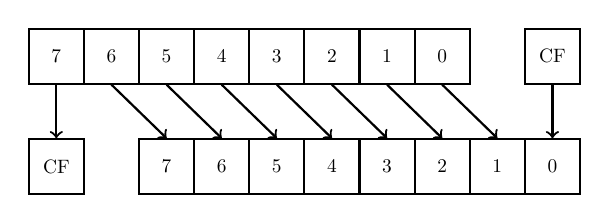
\begin{tikzpicture}[scale=0.7, every node/.style={scale=0.7}]
	\edef\bitsize{1cm}
	\tikzstyle{byte}=[draw,minimum size=\bitsize]
	\tikzstyle{every path}=[thick]

	\node [draw,rectangle,minimum size=\bitsize] (a1) {7};
	\node [draw,rectangle,minimum size=\bitsize] (a2) [right of=a1] {6};
	\node [draw,rectangle,minimum size=\bitsize] (a3) [right of=a2] {5};
	\node [draw,rectangle,minimum size=\bitsize] (a4) [right of=a3] {4};
	\node [draw,rectangle,minimum size=\bitsize] (a5) [right of=a4] {3};
	\node [draw,rectangle,minimum size=\bitsize] (a6) [right of=a5] {2};
	\node [draw,rectangle,minimum size=\bitsize] (a7) [right of=a6] {1};
	\node [draw,rectangle,minimum size=\bitsize] (a8) [right of=a7] {0};
	\node (empty1) [right of=a8] {};
	\node [rectangle,draw,minimum size=\bitsize] (acf) [right of=empty1] {CF};

	\node (empty) [below of=a1] {};

	\node [rectangle,draw,minimum size=\bitsize] (bcf) [below of=empty] {CF};
	\node (empty2) [right of=bcf] {};
	\node [draw,rectangle,minimum size=\bitsize] (b1) [right of=empty2] {7};
	\node [draw,rectangle,minimum size=\bitsize] (b2) [right of=b1] {6};
	\node [draw,rectangle,minimum size=\bitsize] (b3) [right of=b2] {5};
	\node [draw,rectangle,minimum size=\bitsize] (b4) [right of=b3] {4};
	\node [draw,rectangle,minimum size=\bitsize] (b5) [right of=b4] {3};
	\node [draw,rectangle,minimum size=\bitsize] (b6) [right of=b5] {2};
	\node [draw,rectangle,minimum size=\bitsize] (b7) [right of=b6] {1};
	\node [draw,rectangle,minimum size=\bitsize] (b8) [right of=b7] {0};

	\draw [->] (a1.south) -- (bcf.north); % 7
	\draw [->] (a2.south) -- (b1.north); % 6
	\draw [->] (a3.south) -- (b2.north);
	\draw [->] (a4.south) -- (b3.north);
	\draw [->] (a5.south) -- (b4.north);
	\draw [->] (a6.south) -- (b5.north);
	\draw [->] (a7.south) -- (b6.north);
	\draw [->] (a8.south) -- (b7.north);
	\draw [->] (acf.south) -- (b8.north);

	\end{tikzpicture}
\end{center}

  \item[RCR] (M) \RU{вращать биты направо через флаг CF}\EN{rotate right via CF flag}\FR{pivote vers la droite via le flag CF}:

\begin{center}
	\begin{tikzpicture}[scale=0.7, every node/.style={scale=0.7}]
	\edef\bitsize{1cm}
	\tikzstyle{byte}=[draw,minimum size=\bitsize]
	\tikzstyle{every path}=[thick]

	\node [rectangle,draw,minimum size=\bitsize] (acf) {CF};
	\node (empty1) [right of=acf] {};

	\node [draw,rectangle,minimum size=\bitsize] (a1) [right of=empty1] {7};
	\node [draw,rectangle,minimum size=\bitsize] (a2) [right of=a1] {6};
	\node [draw,rectangle,minimum size=\bitsize] (a3) [right of=a2] {5};
	\node [draw,rectangle,minimum size=\bitsize] (a4) [right of=a3] {4};
	\node [draw,rectangle,minimum size=\bitsize] (a5) [right of=a4] {3};
	\node [draw,rectangle,minimum size=\bitsize] (a6) [right of=a5] {2};
	\node [draw,rectangle,minimum size=\bitsize] (a7) [right of=a6] {1};
	\node [draw,rectangle,minimum size=\bitsize] (a8) [right of=a7] {0};

	\node (empty) [below of=a1] {};

	\node [draw,rectangle,minimum size=\bitsize] (b1) [below of=empty] {7};
	\node [draw,rectangle,minimum size=\bitsize] (b2) [right of=b1] {6};
	\node [draw,rectangle,minimum size=\bitsize] (b3) [right of=b2] {5};
	\node [draw,rectangle,minimum size=\bitsize] (b4) [right of=b3] {4};
	\node [draw,rectangle,minimum size=\bitsize] (b5) [right of=b4] {3};
	\node [draw,rectangle,minimum size=\bitsize] (b6) [right of=b5] {2};
	\node [draw,rectangle,minimum size=\bitsize] (b7) [right of=b6] {1};
	\node [draw,rectangle,minimum size=\bitsize] (b8) [right of=b7] {0};

	\node (empty2) [right of=b7] {};

	\node [rectangle,draw,minimum size=\bitsize] (bcf) [right=of empty2] {CF};

	\draw [->] (acf.south) -- (b1.north);
	\draw [->] (a1.south) -- (b2.north);
	\draw [->] (a2.south) -- (b3.north);
	\draw [->] (a3.south) -- (b4.north);
	\draw [->] (a4.south) -- (b5.north);
	\draw [->] (a5.south) -- (b6.north);
	\draw [->] (a6.south) -- (b7.north);
	\draw [->] (a7.south) -- (b8.north);
	\draw [->] (a8.south) -- (bcf.north);

	\end{tikzpicture}
\end{center}


\myindex{x86!\Instructions!ROL}
\myindex{x86!\Instructions!ROR}
\label{ROL_ROR}
\item[ROL/ROR] (M) décalage cyclique

ROL: rotation à gauche:

\begin{center}
	\begin{tikzpicture}[scale=0.7, every node/.style={scale=0.7}]
	\edef\bitsize{1cm}
	\tikzstyle{byte}=[draw,minimum size=\bitsize]	
	\tikzstyle{every path}=[thick]

	\node [draw,rectangle,minimum size=\bitsize] (a1) {7};
	\node [draw,rectangle,minimum size=\bitsize] (a2) [right of=a1] {6};
	\node [draw,rectangle,minimum size=\bitsize] (a3) [right of=a2] {5};
	\node [draw,rectangle,minimum size=\bitsize] (a4) [right of=a3] {4};
	\node [draw,rectangle,minimum size=\bitsize] (a5) [right of=a4] {3};
	\node [draw,rectangle,minimum size=\bitsize] (a6) [right of=a5] {2};
	\node [draw,rectangle,minimum size=\bitsize] (a7) [right of=a6] {1};
	\node [draw,rectangle,minimum size=\bitsize] (a8) [right of=a7] {0};

	\node (empty) [below of=a1] {};

	\node [draw,rectangle,minimum size=\bitsize] (b1) [below of=empty] {7};
	\node [draw,rectangle,minimum size=\bitsize] (b2) [right of=b1] {6};
	\node [draw,rectangle,minimum size=\bitsize] (b3) [right of=b2] {5};
	\node [draw,rectangle,minimum size=\bitsize] (b4) [right of=b3] {4};
	\node [draw,rectangle,minimum size=\bitsize] (b5) [right of=b4] {3};
	\node [draw,rectangle,minimum size=\bitsize] (b6) [right of=b5] {2};
	\node [draw,rectangle,minimum size=\bitsize] (b7) [right of=b6] {1};
	\node [draw,rectangle,minimum size=\bitsize] (b8) [right of=b7] {0};
	
	\node [shape=rectangle,draw,minimum size=\bitsize] (cf) [left=of b1] {CF};
	
	\draw [->] (a1.south) -- (b8.north);
	\draw [->] (a2.south) -- (b1.north);
	\draw [->] (a3.south) -- (b2.north);
	\draw [->] (a4.south) -- (b3.north);
	\draw [->] (a5.south) -- (b4.north);
	\draw [->] (a6.south) -- (b5.north);
	\draw [->] (a7.south) -- (b6.north);
	\draw [->] (a8.south) -- (b7.north);
	
	\draw [->] (a1.south) -- (cf.north);

	\end{tikzpicture}
\end{center}



ROR: rotation à droite:

\begin{center}
	\begin{tikzpicture}[scale=0.7, every node/.style={scale=0.7}]
	\edef\bitsize{1cm}
	\tikzstyle{byte}=[draw,minimum size=\bitsize]	
	\tikzstyle{every path}=[thick]

	\node [draw,rectangle,minimum size=\bitsize] (a1) {7};
	\node [draw,rectangle,minimum size=\bitsize] (a2) [right of=a1] {6};
	\node [draw,rectangle,minimum size=\bitsize] (a3) [right of=a2] {5};
	\node [draw,rectangle,minimum size=\bitsize] (a4) [right of=a3] {4};
	\node [draw,rectangle,minimum size=\bitsize] (a5) [right of=a4] {3};
	\node [draw,rectangle,minimum size=\bitsize] (a6) [right of=a5] {2};
	\node [draw,rectangle,minimum size=\bitsize] (a7) [right of=a6] {1};
	\node [draw,rectangle,minimum size=\bitsize] (a8) [right of=a7] {0};

	\node (empty) [below of=a1] {};

	\node [draw,rectangle,minimum size=\bitsize] (b1) [below of=empty] {7};
	\node [draw,rectangle,minimum size=\bitsize] (b2) [right of=b1] {6};
	\node [draw,rectangle,minimum size=\bitsize] (b3) [right of=b2] {5};
	\node [draw,rectangle,minimum size=\bitsize] (b4) [right of=b3] {4};
	\node [draw,rectangle,minimum size=\bitsize] (b5) [right of=b4] {3};
	\node [draw,rectangle,minimum size=\bitsize] (b6) [right of=b5] {2};
	\node [draw,rectangle,minimum size=\bitsize] (b7) [right of=b6] {1};
	\node [draw,rectangle,minimum size=\bitsize] (b8) [right of=b7] {0};
	
	\node [shape=rectangle,draw,minimum size=\bitsize] (cf) [right=of b7] {CF};
	
	\draw [->] (a1.south) -- (b2.north);
	\draw [->] (a2.south) -- (b3.north);
	\draw [->] (a3.south) -- (b4.north);
	\draw [->] (a4.south) -- (b5.north);
	\draw [->] (a5.south) -- (b6.north);
	\draw [->] (a6.south) -- (b7.north);
	\draw [->] (a7.south) -- (b8.north);
	\draw [->] (a8.south) -- (b1.north);
	
	\draw [->] (a8.south) -- (cf.north);

	\end{tikzpicture}
\end{center}



En dépit du fait que presque presque tous les \ac{CPU}s aient ces instructions, il n'y
a pas d'opération correspondante en \CCpp, donc les compilateurs de ces \ac{PL}s
ne génèrent en général pas ces instructions.

Par commodité pour le programmeur, au moins \ac{MSVC} fourni les pseudo-fonctions
(fonctions intrinsèques du compilateur)
\emph{\_rotl()} et \emph{\_rotr()}\FNMSDNROTxURL{},
qui sont traduites directement par le compilateur en ces instructions.


\myindex{x86!\Instructions!SAL}
  \item[SAL] \RU{Арифметический сдвиг влево}\EN{Arithmetic shift left}\FR{Décalage
  arithmétique à gauche}, \RU{синонимично}\EN{synonymous to}\FR{synonyme de} \TT{SHL}

\myindex{x86!\Instructions!SAR}
  \label{ins:SAR}
  \item[SAR] \RU{Арифметический сдвиг вправо}\EN{Arithmetic shift right}\FR{Décalage arithmétique à droite}

\begin{center}
	\begin{tikzpicture}[scale=0.7, every node/.style={scale=0.7}]
	\edef\bitsize{1cm}
	\tikzstyle{byte}=[draw,minimum size=\bitsize]
	\tikzstyle{every path}=[thick]

	\node [draw,rectangle,minimum size=\bitsize] (a1) {7};
	\node [draw,rectangle,minimum size=\bitsize] (a2) [right of=a1] {6};
	\node [draw,rectangle,minimum size=\bitsize] (a3) [right of=a2] {5};
	\node [draw,rectangle,minimum size=\bitsize] (a4) [right of=a3] {4};
	\node [draw,rectangle,minimum size=\bitsize] (a5) [right of=a4] {3};
	\node [draw,rectangle,minimum size=\bitsize] (a6) [right of=a5] {2};
	\node [draw,rectangle,minimum size=\bitsize] (a7) [right of=a6] {1};
	\node [draw,rectangle,minimum size=\bitsize] (a8) [right of=a7] {0};

	\node (empty) [below of=a1] {};

	\node [draw,rectangle,minimum size=\bitsize] (b1) [below of=empty] {7};
	\node [draw,rectangle,minimum size=\bitsize] (b2) [right of=b1] {6};
	\node [draw,rectangle,minimum size=\bitsize] (b3) [right of=b2] {5};
	\node [draw,rectangle,minimum size=\bitsize] (b4) [right of=b3] {4};
	\node [draw,rectangle,minimum size=\bitsize] (b5) [right of=b4] {3};
	\node [draw,rectangle,minimum size=\bitsize] (b6) [right of=b5] {2};
	\node [draw,rectangle,minimum size=\bitsize] (b7) [right of=b6] {1};
	\node [draw,rectangle,minimum size=\bitsize] (b8) [right of=b7] {0};

	\node [shape=rectangle,draw,minimum size=\bitsize] (cf) [right=of b7] {CF};

	\draw [->] (a1.south) -- (b1.north); %7
	\draw [->] (a1.south) -- (b2.north); %6

	\draw [->] (a2.south) -- (b3.north); %6
	\draw [->] (a3.south) -- (b4.north); %5
	\draw [->] (a4.south) -- (b5.north); %4
	\draw [->] (a5.south) -- (b6.north); %3
	\draw [->] (a6.south) -- (b7.north); %2
	\draw [->] (a7.south) -- (b8.north); %1

	\draw [->] (a8.south) -- (cf.north);

	\end{tikzpicture}
\end{center}

\RU{Таким образом, бит знака всегда остается на месте}%
\EN{Hence, the sign bit always stays at the place of the}%
\FR{De ce fait, le bit de signe reste toujours à la place du} \ac{MSB}.


\myindex{x86!\Instructions!SETcc}
  \item[SETcc] op: \RU{загрузить 1 в op (только байт) если условие верно или 0 если наоборот}%
  \EN{load 1 to operand (byte only) if the condition is true or zero otherwise}%
  \FR{charge 1 dans l'opérande (octet seulement) si la condition est vraie et zéro sinon}.
  \RU{Коды точно такие же, как и в инструкциях Jcc}\EN{The condition codes are the same as in the Jcc instructions}%
  \FR{Les codes conditions sont les même que les instructions Jcc}
  (\myref{Jcc}).


\myindex{x86!\Instructions!STC}
\myindex{x86!\Flags!CF}
  \item[STC] (M) \RU{установить флаг CF}\EN{set CF flag}\FR{met le flag CF}

\myindex{x86!\Instructions!STD}
\myindex{x86!\Flags!DF}
  \item[STD] (M) Met le flag DF.
   Cette instruction n'est pas générée par les compilateurs et est en général rare.
   Par exemple, elle peut être trouvée dans le fichier du noyau de Windows \TT{ntoskrnl.exe},
   dans la routine de copie mémoire écrite à la main.

\myindex{x86!\Instructions!STI}
\myindex{x86!\Flags!IF}
  \item[STI] (M) \RU{установить флаг IF}\EN{set IF flag}\FR{met le flag IF}

\myindex{x86!\Instructions!SYSCALL}
  \item[SYSCALL] (AMD) \RU{вызов сисколла}\EN{call syscall}\FR{appelle un appel système} (\myref{syscalls})

\myindex{x86!\Instructions!SYSENTER}
  \item[SYSENTER] (Intel) \RU{вызов сисколла}\EN{call syscall}\FR{appel un appel système} (\myref{syscalls})

\myindex{x86!\Instructions!UD2}
  \item[UD2] (M) \RU{неопределенная инструкция, вызывает исключение. Применяется для тестирования.}
  \EN{undefined instruction, raises exception. Used for testing.}\FR{instruction
  indéfinie, lève une exception. Utilisée pour tester.}

\myindex{x86!\Instructions!XCHG}
  \item[XCHG] (M) \RU{обменять местами значения в операндах}\EN{exchange the values in the operands}%
\FR{échange les valeurs dans les opérandes}

\myindex{Borland Delphi}
\RU{Это редкая инструкция: компиляторы её не генерируют, потому что начиная с Pentium, XCHG с адресом в памяти в операнде
исполняется так, как если имеет префикс LOCK (см.\InSqBrackets{\MAbrash глава 19}).
Вероятно, в Intel так сделали для совместимости с синхронизирующими примитивами.
Таким образом, XCHG начиная с Pentium может быть медленной.
С другой стороны, XCHG была очень популярна у программистов на ассемблере.
Так что, если вы видите XCHG в коде, это может быть знаком, что код написан вручную.
Впрочем, по крайней мере компилятор Borland Delphi генерирует эту инструкцию.}
\EN{This instruction is rare: compilers don't generate it, because starting at Pentium, XCHG with address in memory in operand executes as if it has LOCK prefix (\InSqBrackets{\MAbrash chapter 19}).
Perhaps, Intel engineers did so for compatibility with synchronizing primitives.
Hence, XCHG starting at Pentium can be slow.
On the other hand, XCHG was very popular in assembly language programmers.
So if you see XCHG in code, it can be a sign that this piece of code is written manually.
However, at least Borland Delphi compiler generates this instruction.}
\FR{Cette instruction est rare: les compilateurs ne la génère pas, car à partir du
Pentium, XCHG avec comme opérande une adresse en mémoire s'exécute comme si elle
avait le préfixe LOCK (\InSqBrackets{\MAbrash chapter 19}).
Peut-être que les ingénieurs d'Intel ont fait cela pour la compatibilité avec les
primitives de synchronisation.
Ainsi, à partir du Pentium, XCHG peut être lente.
D'un autre côté, XCHG était très populaire chez les programmeurs en langage d'assemblage.
Donc, si vous voyez XCHG dans le code, ça peut être un signe que ce morceau de code
a été écrit à la main.
Toutefois, au moins le compilateur Borland Delphi génère cette instruction.}


\end{description}

\subsubsection{Instructions FPU}

Le suffixe \TT{-R} dans le mnémonique signifie en général que les opérandes sont
inversés, le suffixe \TT{-P} implique qu'un élément est supprimé de la pile après
l'exécution de l'instruction, le suffixe \TT{-PP} implique que deux éléments sont
supprimés.

Les instructions \TT{-P} sont souvent utiles lorsque nous n'avons plus besoin que
la valeur soit présente dans la pile FPU après l'opération.

\begin{description}
\myindex{x86!\Instructions!FABS}
  \item[FABS] \RU{заменить значение в ST(0) на абсолютное значение ST(0)}\EN{replace value in ST(0) by absolute value in ST(0)}%
  \FR{remplace la valeur dans ST(0) par sa valeur absolue}

\myindex{x86!\Instructions!FADD}
\myindex{x86!\Instructions!FADDP}
  \item[FADD] op: ST(0)=op+ST(0)
  \item[FADD] ST(0), ST(i): ST(0)=ST(0)+ST(i)
  \item[FADDP] ST(1)=ST(0)+ST(1);
  \RU{вытолкнуть один элемент из стека, таким образом, складываемые значения в стеке заменяются
  суммой}\EN{pop one element from the stack, i.e., the values in the stack are replaced by their sum}%
  \FR{supprime un élément de la pile, i.e., les valeurs sur la pile sont remplacées par leurs somme}

 % + FADDP
\myindex{x86!\Instructions!FCHS}
  \item[FCHS] ST(0)=-ST(0)


\myindex{x86!\Instructions!FCOM}
\myindex{x86!\Instructions!FCOMP}
\myindex{x86!\Instructions!FCOMPP}
  \item[FCOM] compare ST(0) avec ST(1)
  \item[FCOM] op: compare ST(0) avec op
  \item[FCOMP] compare ST(0) avec ST(1); supprime un élément de la pile
  \item[FCOMPP] compare ST(0) avec ST(1); supprime deux éléments de la pile

 % + FCOMP + FCOMPP
\myindex{x86!\Instructions!FDIVR}
\myindex{x86!\Instructions!FDIVRP}
  \item[FDIVR] op: ST(0)=op/ST(0)
  \item[FDIVR] ST(i), ST(j): ST(i)=ST(j)/ST(i)
  \item[FDIVRP] op: ST(0)=op/ST(0); \RU{вытолкнуть один элемент из стека}\EN{pop one element from the stack}%
  \FR{supprime un élément de la pile}
  \item[FDIVRP] ST(i), ST(j): ST(i)=ST(j)/ST(i); \RU{вытолкнуть один элемент из стека}\EN{pop one element from the stack}%
  \FR{supprime un élément de la pile}

 % + FDIVRP
\myindex{x86!\Instructions!FDIV}
\myindex{x86!\Instructions!FDIVP}
  \item[FDIV] op: ST(0)=ST(0)/op
  \item[FDIV] ST(i), ST(j): ST(i)=ST(i)/ST(j)
  \item[FDIVP] ST(1)=ST(0)/ST(1); \RU{вытолкнуть один элемент из стека, таким образом,
  делимое и делитель в стеке заменяются частным}\EN{pop one element from the stack, i.e.,
  the dividend and divisor values in the stack are replaced by quotient}\FR{supprime un
  élément de la pile, i.e, les valeurs du dividende et du diviseur sont remplacées par
  le quotient}
 % + FDIVP
\myindex{x86!\Instructions!FILD}
  \item[FILD] op: \RU{сконвертировать целочисленный op и затолкнуть его в стек}
  \EN{convert integer and push it to the stack}\FR{convertit un entier n et le pousse sur la pile}.


\myindex{x86!\Instructions!FIST}
\myindex{x86!\Instructions!FISTP}
  \item[FIST] op: convertit la valeur dans ST(0) en un entier dans op
  \item[FISTP] op: convertit la valeur dans ST(0) en un entier dans op;
  supprime un élément de la pile
 % + FISTP
\myindex{x86!\Instructions!FLD1}
  \item[FLD1] \RU{затолкнуть 1 в стек}\EN{push 1 to stack}\FR{pousse 1 sur la pile}


\myindex{x86!\Instructions!FLDCW}
  \item[FLDCW] op: \RU{загрузить}\EN{load}\FR{charge le} FPU control word (\myref{FPU_control_word}) \RU{из}\EN{from}\FR{depuis le} 16-bit op.


\myindex{x86!\Instructions!FLDZ}
  \item[FLDZ] \RU{затолкнуть ноль в стек}\EN{push zero to stack}\FR{pousse zéro sur la pile}



\myindex{x86!\Instructions!FLD}
  \item[FLD] op: \RU{затолкнуть op в стек}\EN{push op to the stack}\FR{pousse op sur la pile}.

\myindex{x86!\Instructions!FMUL}
\myindex{x86!\Instructions!FMULP}
  \item[FMUL] op: ST(0)=ST(0)*op
  \item[FMUL] ST(i), ST(j): ST(i)=ST(i)*ST(j)
  \item[FMULP] op: ST(0)=ST(0)*op; \RU{вытолкнуть один элемент из стека}\EN{pop one element from the stack}%
  \FR{supprime un élément de la pile}
  \item[FMULP] ST(i), ST(j): ST(i)=ST(i)*ST(j); \RU{вытолкнуть один элемент из стека}\EN{pop one element from the stack}%
  \FR{supprime un élément de la pile}

 % + FMULP
\myindex{x86!\Instructions!FSINCOS}
  \item[FSINCOS]: tmp=ST(0); ST(1)=sin(tmp); ST(0)=cos(tmp)


\myindex{x86!\Instructions!FSQRT}
  \item[FSQRT]: $ST(0)=\sqrt{ST(0)}$


\myindex{x86!\Instructions!FSTCW}
\myindex{x86!\Instructions!FNSTCW}
  \item[FSTCW] op: stocker le mot de contrôle FPU (\myref{FPU_control_word}) dans l'op 16-bit
  après avoir vérifié s'il y a des exceptions en attente.
  \item[FNSTCW] op: stocker le mot de contrôle FPU (\myref{FPU_control_word}) dans l'op 16-bit.

 % + FNSTCW
\myindex{x86!\Instructions!FSTSW}
\myindex{x86!\Instructions!FNSTSW}
  \item[FSTSW] op: stocker le mot d'état FPU (\myref{FPU_status_word}) dans l'op 16-bit
  après avoir vérifié s'il y a des exceptions en attente.
  \item[FNSTSW] op: stocker le mot d'état FPU (\myref{FPU_status_word}) dans l'op 16-bit.

 % + FNSTSW
\myindex{x86!\Instructions!FST}
\myindex{x86!\Instructions!FSTP}
  \item[FST] op: \RU{копировать}\EN{copy}\FR{copie} ST(0) \RU{в}\EN{to}\FR{dans} op
  \item[FSTP] op: \RU{копировать}\EN{copy}\FR{copie} ST(0) \RU{в}\EN{to}\FR{dans} op;
  \RU{вытолкнуть один элемент из стека}\EN{pop one element from the stack}%
  \FR{supprime un élément de la pile}

\myindex{x86!\Instructions!FSUBR}
\myindex{x86!\Instructions!FSUBRP}
  \item[FSUBR] op: ST(0)=op-ST(0)
  \item[FSUBR] ST(0), ST(i): ST(0)=ST(i)-ST(0)
  \item[FSUBRP] ST(1)=ST(0)-ST(1);
  \RU{вытолкнуть один элемент из стека, таким образом, складываемые значения в стеке заменяются
  разностью}\EN{pop one element from the stack, i.e., the value in the stack is replaced by the difference}%
  \FR{supprime un élément de la pile, i.e., la valeur dans la pile est remplacée par la différence}

 % + FSUBRP
\myindex{x86!\Instructions!FSUB}
\myindex{x86!\Instructions!FSUBP}
  \item[FSUB] op: ST(0)=ST(0)-op
  \item[FSUB] ST(0), ST(i): ST(0)=ST(0)-ST(i)
  \item[FSUBP] ST(1)=ST(1)-ST(0);
  \RU{вытолкнуть один элемент из стека, таким образом, складываемые значения в стеке заменяются
  разностью}\EN{pop one element from the stack, i.e., the value in the stack is replaced by the difference}%
  \FR{supprime un élément de la pile, i.e., la valeur dans la pile est remplacée par la différence}

 % + FSUBP
\myindex{x86!\Instructions!FUCOM}
\myindex{x86!\Instructions!FUCOMP}
\myindex{x86!\Instructions!FUCOMPP}
  \item[FUCOM] ST(i): compare ST(0) et ST(i)
  \item[FUCOM] compare ST(0) et ST(1)
  \item[FUCOMP] compare ST(0) et ST(1); supprime un élément de la pile.
  \item[FUCOMPP] compare ST(0) et ST(1); supprime deux éléments de la pile.

  L'instruction se comporte comme FCOM, mais une exception est levée seulement si
  un opérande est SNaN, tandis que les nombres QNaN sont traités normalement.
 % + FUCOMP + FUCOMPP
\myindex{x86!\Instructions!FXCH}
  \item[FXCH] ST(i) \RU{обменять местами значения в ST(0) и ST(i)}\EN{exchange values in ST(0) and ST(i)}%
  \FR{échange les valeurs dans ST(0) et ST(i)}
  \item[FXCH] \RU{обменять местами значения в ST(0) и ST(1)}\EN{exchange values in ST(0) and ST(1)}%
  \FR{échange les valeurs dans ST(0) et ST(1)}


\end{description}

%\subsubsection{\RU{SIMD-инструкции}\EN{SIMD instructions}}

% TODO

%\begin{description}
%\input{appendix/x86/instructions/DIVSD}
%\input{appendix/x86/instructions/MOVDQA}
%\input{appendix/x86/instructions/MOVDQU}
%\input{appendix/x86/instructions/PADDD}
%\input{appendix/x86/instructions/PCMPEQB}
%\input{appendix/x86/instructions/PLMULHW}
%\input{appendix/x86/instructions/PLMULLD}
%\input{appendix/x86/instructions/PMOVMSKB}
%\input{appendix/x86/instructions/PXOR}
%\end{description}

% SHLD !
% SHRD !
% BSWAP !
% CMPXCHG
% XADD !
% CMPXCHG8B
% RDTSC !
% PAUSE!

% xsave
% fnclex, fnsave
% movsxd, movaps, wait, sfence, lfence, pushfq
% prefetchw
% REP RETN
% REP BSF
% movnti, movntdq, rdmsr, wrmsr
% ldmxcsr, stmxcsr, invlpg
% swapgs
% movq, movd
% mulsd
% POR
% IRETQ
% pslldq
% psrldq
% cqo, fxrstor, comisd, xrstor, wbinvd, movntq
% fprem
% addsb, subsd, frndint

% rare:
%\item[ENTER]
%\item[LES]
% LDS
% XLAT

\subsubsection{Instructions ayant un opcode affichable en ASCII}

(En mode 32-bit.)

\label{printable_x86_opcodes}
\myindex{Shellcode}
Elles peuvent être utilisées pour la création de shellcode.
Voir aussi: \myref{subsec:EICAR}.

% FIXME: start at 0x20...
\begin{center}
\begin{longtable}{ | l | l | l | }
\hline
\HeaderColor caractère ASCII & 
\HeaderColor code hexadécimal & 
\HeaderColor instruction x86 \\
\hline
0	 &30	 &XOR \\
1	 &31	 &XOR \\
2	 &32	 &XOR \\
3	 &33	 &XOR \\
4	 &34	 &XOR \\
5	 &35	 &XOR \\
7	 &37	 &AAA \\
8	 &38	 &CMP \\
9	 &39	 &CMP \\
:	 &3a	 &CMP \\
;	 &3b	 &CMP \\
<	 &3c	 &CMP \\
=	 &3d	 &CMP \\
?	 &3f	 &AAS \\
@	 &40	 &INC \\
A	 &41	 &INC \\
B	 &42	 &INC \\
C	 &43	 &INC \\
D	 &44	 &INC \\
E	 &45	 &INC \\
F	 &46	 &INC \\
G	 &47	 &INC \\
H	 &48	 &DEC \\
I	 &49	 &DEC \\
J	 &4a	 &DEC \\
K	 &4b	 &DEC \\
L	 &4c	 &DEC \\
M	 &4d	 &DEC \\
N	 &4e	 &DEC \\
O	 &4f	 &DEC \\
P	 &50	 &PUSH \\
Q	 &51	 &PUSH \\
R	 &52	 &PUSH \\
S	 &53	 &PUSH \\
T	 &54	 &PUSH \\
U	 &55	 &PUSH \\
V	 &56	 &PUSH \\
W	 &57	 &PUSH \\
X	 &58	 &POP \\
Y	 &59	 &POP \\
Z	 &5a	 &POP \\
\lbrack{}	 &5b	 &POP \\
\textbackslash{}	 &5c	 &POP \\
\rbrack{}	 &5d	 &POP \\
\verb|^|	 &5e	 &POP \\
\_	 &5f	 &POP \\
\verb|`|	 &60	 &PUSHA \\
a	 &61	 &POPA \\
f	 &66	 &en mode 32-bit, change pour une\\
   & & taille d'opérande de 16-bit \\
g	 &67	 &en mode 32-bit, change pour une\\
   & & taille d'adresse 16-bit \\
h	 &68	 &PUSH\\
i	 &69	 &IMUL\\
j	 &6a	 &PUSH\\
k	 &6b	 &IMUL\\
p	 &70	 &JO\\
q	 &71	 &JNO\\
r	 &72	 &JB\\
s	 &73	 &JAE\\
t	 &74	 &JE\\
u	 &75	 &JNE\\
v	 &76	 &JBE\\
w	 &77	 &JA\\
x	 &78	 &JS\\
y	 &79	 &JNS\\
z	 &7a	 &JP\\
\hline
\end{longtable}
\end{center}

De même:
\begin{center}
\begin{longtable}{ | l | l | l | }
\hline
\HeaderColor caractère ASCII & 
\HeaderColor code hexadécimal & 
\HeaderColor instruction x86 \\
\hline
f	 &66	 &en mode 32-bit, change pour une\\
   & & taille d'opérande de 16-bit \\
g	 &67	 &en mode 32-bit, change pour une\\
   & & taille d'adresse 16-bit \\
\hline
\end{longtable}
\end{center}

\myindex{x86!\Instructions!AAA}
\myindex{x86!\Instructions!AAS}
\myindex{x86!\Instructions!CMP}
\myindex{x86!\Instructions!DEC}
\myindex{x86!\Instructions!IMUL}
\myindex{x86!\Instructions!INC}
\myindex{x86!\Instructions!JA}
\myindex{x86!\Instructions!JAE}
\myindex{x86!\Instructions!JB}
\myindex{x86!\Instructions!JBE}
\myindex{x86!\Instructions!JE}
\myindex{x86!\Instructions!JNE}
\myindex{x86!\Instructions!JNO}
\myindex{x86!\Instructions!JNS}
\myindex{x86!\Instructions!JO}
\myindex{x86!\Instructions!JP}
\myindex{x86!\Instructions!JS}
\myindex{x86!\Instructions!POP}
\myindex{x86!\Instructions!POPA}
\myindex{x86!\Instructions!PUSH}
\myindex{x86!\Instructions!PUSHA}
\myindex{x86!\Instructions!XOR}

En résumé:
AAA, AAS, CMP, DEC, IMUL, INC, JA, JAE, JB, JBE, JE, JNE, JNO, JNS, JO, JP, JS, POP, POPA, PUSH, PUSHA, 
XOR.


\mysection{Patterns de code suspect}

\subsection{instructions XOR}
\myindex{x86!\Instructions!XOR}

Des instructions comme \TT{XOR op, op} (par exemple, \TT{XOR EAX, EAX}) sont utilisées
en général pour mettre la valeur d'un registre à zéro, mais si les opérandes sont
différentes, l'opération \q{ou exclusif} est exécutée.

Cette opération est rare en programmation courante, mais répandu en cryptographie,
y compris amateur.
C'est particulièrement suspect si le second opérande est un grand nombre.

Ceci peut indiquer du chiffrement/déchiffrement, du calcul de somme de contrôle, etc.\\
\\

Une exception à cette observation, qu'il est utile de noter, est le \q{canari} (\myref{subsec:BO_protection}).
Sa génération et sa vérification sont souvent effectuées en utilisant des instructions
\XOR. \\
\\
\myindex{AWK}

Ce script awk peut être utilisé pour traité les fichiers listing (.lst) d'\IDA:

\lstinputlisting{digging_into_code/awk.sh}

Il est aussi utile de noter que ce type de script peut aussi rapporter du code mal
désassemblé
(\myref{sec:incorrectly_disasmed_code}).

\subsection{Code assembleur écrit à la main}

\myindex{Function prologue}
\myindex{Function epilogue}
\myindex{x86!\Instructions!LOOP}
\myindex{x86!\Instructions!RCL}

Les compilateurs modernes ne génèrent pas les instructions \TT{LOOP} et \TT{RCL}.
D'un autre côté, ces instructions sont très connues des codeurs qui aiment écrire
directement en langage d'assemblage.
Si vous les rencontrez, on peut dire qu'il est très probable que ce morceau de code
ait été écrit à la main.
De telles instructions sont marquées avec un (M) dans la liste des instructions de
cet appendice: \myref{sec:x86_instructions}.

\par
De même, les prologue/épilogue de fonction sont rares dans de l'assembleur écrit
à la main.

\par
Il n'y a généralement pas de système fixé pour le passage des arguments aux fonctions
dans du code écrit à la main.

\par
Exemple du noyau de Windows 2003
(ntoskrnl.exe file):

\lstinputlisting[style=customasmx86]{digging_into_code/ntoskrnl.lst}

En effet, si nous regardons dans le code source de \ac{WRK} v1.2, ce code peut être
trouvé facilement dans le fichier \\
\emph{WRK-v1.2\textbackslash{}base\textbackslash{}ntos\textbackslash{}ke\textbackslash{}i386\textbackslash{}cpu.asm}.

\par 
D'après l'instruction \INS{RCL} que j'ai pu trouver dans le fichier ntoskrnl.exe de Windows
2003 x86 (compilé avec MS Visual C compiler).
Elle apparaît seulement une fois ici, \\
dans la fonction \TT{RtlExtendedLargeIntegerDivide()}
et ça pourrait être un cas de code assembleur en ligne.

\mysection{Utilisation de nombres magiques lors du tracing}

Souvent, notre but principal est de comprendre comment le programme utilise une valeur
qui a été soit lue d'un fichier ou reçue par le réseau. Le tracing manuel d'une valeur
est souvent une tâche laborieuse. Une des techniques les plus simple pour ceci (bien
que non sûre à 100\%) est d'utiliser votre propre \emph{nombre magique}.

Ceci ressemble à la tomodensitométrie aux rayons X: un agent de radio-contraste est
injecté dans le sang du patient, qui est utilisé pour augmenter la visibilité de
la structure interne du patient aux rayons X.
C'est bien connu comment le sang circule dans les reins d'humains en bonne santé
et si l'agent est dans le sang, il peut être vu facilement en tomographie comment
le sang circule et si il y a des calculs ou des tumeurs.

Nous pouvons prendre un nombre 32-bit comme \TT{0x0badf00d}, ou la date de naissance
de quelqu'un comme \TT{0x11101979} et écrire ce nombre de 4 octets quelque part dans
un fichier utilisé par le programme que nous investiguons.

\myindex{\GrepUsage}
\myindex{tracer}

Puis, en suivant ce programme avec \tracer en mode \emph{code coverage}, avec l'aide
de \emph{grep} ou simplement en cherchant dans le fichier texte (résultant de l'investigation),
nous pouvons facilement voir où la valeur a été utilisée et comment.

Exemple de résultats de \tracer \emph{grepable} en mode \emph{cc}:

\begin{lstlisting}[style=customasmx86]
0x150bf66 (_kziaia+0x14), e=       1 [MOV EBX, [EBP+8]] [EBP+8]=0xf59c934
0x150bf69 (_kziaia+0x17), e=       1 [MOV EDX, [69AEB08h]] [69AEB08h]=0
0x150bf6f (_kziaia+0x1d), e=       1 [FS: MOV EAX, [2Ch]]
0x150bf75 (_kziaia+0x23), e=       1 [MOV ECX, [EAX+EDX*4]] [EAX+EDX*4]=0xf1ac360
0x150bf78 (_kziaia+0x26), e=       1 [MOV [EBP-4], ECX] ECX=0xf1ac360
\end{lstlisting}
% TODO: good example!

Cela peut aussi être utilisé pour des paquets réseau.
Il est important que le \emph{nombre magique} soit unique et ne soit pas présent
dans le code du programme.

\newcommand{\DOSBOXURL}{\href{http://blog.yurichev.com/node/55}{blog.yurichev.com}}

\myindex{DosBox}
\myindex{MS-DOS}
À part \tracer, DosBox (émulateur MS-DOS) en mode heavydebug est capable d'écrire
de l'information à propos de l'état de tous les registres pour chaque instruction
du programme exécutée dans un fichier texte\footnote{Voir aussi mon article de blog
sur cette fonctionnalité de DosBox: \DOSBOXURL{}}, donc cette technique peut être
utile également pour des programmes DOS.

\mysection{Boucles}

À chaque fois que votre programme travaille avec des sortes de fichier, ou un buffer
d'une certaine taille, il doit s'agir d'un sorte de boucle de déchiffrement/traitement
à l'intérieur du code.

Ceci est un exemple réel de sortie de l'outil \tracer.
Il y avait un code qui chargeait une sorte de fichier chiffré de 258 octets.
Je l'ai lancé dans l'intention d'obtenir le nombre d'exécution de chaque instruction
(l'outil \ac{DBI} irait beaucoup mieux de nos jours).
Et j'ai rapidement trouvé un morceau de code qui était exécuté 259/258 fois:

\lstinputlisting{digging_into_code/crypto_loop.txt}

Il s'avère qu'il s'agit de la boucle de déchiffrement.


\subsection{Exemple \#2: SCO OpenServer}

\label{examples_SCO}
\myindex{SCO OpenServer}
Un ancien logiciel pour SCO OpenServer de 1997 développé par une société qui a disparue
depuis longtemps.

Il y a un driver de dongle special à installer dans le système, qui contient les
chaînes de texte suivantes:
\q{Copyright 1989, Rainbow Technologies, Inc., Irvine, CA}
et
\q{Sentinel Integrated Driver Ver. 3.0 }.

Après l'installation du driver dans SCO OpenServer, ces fichiers apparaissent dans
l'arborescence /dev:

\begin{lstlisting}
/dev/rbsl8
/dev/rbsl9
/dev/rbsl10
\end{lstlisting}

Le programme renvoie une erreur lorsque le dongle n'est pas connecté, mais le message
d'erreur n'est pas trouvé dans les exécutables.

\myindex{COFF}

Grâce à \ac{IDA}, il est facile de charger l'exécutable COFF utilisé dans SCO OpenServer.

Essayons de trouver la chaîne \q{rbsl} et en effet, elle se trouve dans ce morceau
de code:

\lstinputlisting[style=customasmx86]{examples/dongles/2/1.lst}

Oui, en effet, le programme doit communiquer d'une façon ou d'une autre avec le driver.

\myindex{thunk-functions}
Le seul endroit où la fonction \TT{SSQC()} est appelée est dans la \glslink{thunk
 function}{fonction thunk}:

\lstinputlisting[style=customasmx86]{examples/dongles/2/2.lst}

SSQ() peut être appelé depuis au moins 2 fonctions.

L'une d'entre elles est:

\lstinputlisting[style=customasmx86]{examples/dongles/2/check1_EN.lst}

\q{\TT{3C}} et \q{\TT{3E}} semblent familiers: il y avait un dongle Sentinel Pro de
Rainbow sans mémoire, fournissant seulement une fonction de crypto-hachage secrète.

Vous pouvez lire une courte description de la fonction de hachage dont il s'agit
ici: \myref{hash_func}.

Mais retournons au programme.

Donc le programme peut seulement tester si un dongle est connecté ou s'il est absent.

Aucune autre information ne peut être écrite dans un tel dongle, puisqu'il n'a pas
de mémoire.
Les codes sur deux caractères sont des commandes (nous pouvons voir comment les commandes
sont traitées dans la fonction \TT{SSQC()}) et toutes les autres chaînes sont hachées
dans le dongle, transformées en un nombre 16-bit.
L'algorithme était secret, donc il n'était pas possible d'écrire un driver de remplacement
ou de refaire un dongle matériel qui l'émulerait parfaitement.

Toutefois, il est toujours possible d'intercepter tous les accès au dongle et de
trouver les constantes auxquelles les résultats de la fonction de hachage sont comparées.

Mais nous devons dire qu'il est possible de construire un schéma de logiciel de protection
de copie robuste basé sur une fonction secrète de hachage cryptographique: il suffit
qu'elle chiffre/déchiffre les fichiers de données utilisés par votre logiciel.

Mais retournons au code:

Les codes 51/52/53 sont utilisés pour choisir le port imprimante LPT.
3x/4x sont utilisés pour le choix de la \q{famille} (c'est ainsi que les dongles
Sentinel Pro sont différenciés les uns des autres: plus d'un dongle peut être connecté
sur un port LPT).

La seule chaîne passée à la fonction qui ne fasse pas 2 caractères est "0123456789".

Ensuite, le résultat est comparé à l'ensemble des résultats valides.

Si il est correct, 0xC ou 0xB est écrit dans la variable globale \TT{ctl\_model}.%

Une autre chaîne de texte qui est passée est
"PRESS ANY KEY TO CONTINUE: ", mais le résultat n'est pas testé.
Difficile de dire pourquoi, probablement une erreur\footnote{C'est un sentiment
étrange de trouver un bug dans un logiciel aussi ancien.}.

Voyons où la valeur de la variable globale \TT{ctl\_model} est utilisée.

Un tel endroit est:

\lstinputlisting[style=customasmx86]{examples/dongles/2/4.lst}

Si c'est 0, un message d'erreur chiffré est passé à une routine de déchiffrement
et affiché.

\myindex{x86!\Instructions!XOR}

La routine de déchiffrement de la chaîne semble être un simple \glslink{xoring}{xor}:

\lstinputlisting[style=customasmx86]{examples/dongles/2/err_warn.lst}

C'est pourquoi nous étions incapable de trouver le message d'erreur dans les fichiers
exécutable, car ils sont chiffrés (ce qui est une pratique courante).

Un autre appel à la fonction de hachage \TT{SSQ()} lui passe la chaîne \q{offln}
et le résultat est comparé avec \TT{0xFE81} et \TT{0x12A9}.

Si ils ne correspondent pas, ça se comporte comme une sorte de fonction \TT{timer()}
(peut-être en attente qu'un dongle mal connecté soit reconnecté et re-testé?) et ensuite
déchiffre un autre message d'erreur à afficher.

\lstinputlisting[style=customasmx86]{examples/dongles/2/check2_EN.lst}

Passer outre le dongle est assez facile: il suffit de patcher tous les sauts après
les instructions \CMP pertinentes.

Une autre option est d'écrire notre propre driver SCO OpenServer, contenant une table
de questions et de réponses, toutes celles qui sont présentent dans le programme.

\subsubsection{Déchiffrer les messages d'erreur}

À propos, nous pouvons aussi essayer de déchiffrer tous les messages d'erreurs.
L'algorithme qui se trouve dans la fonction \TT{err\_warn()} est très simple, en effet:

\lstinputlisting[caption=Decryption function,style=customasmx86]{examples/dongles/2/decrypting_FR.lst}

Comme on le voit, non seulement la chaîne est transmise à la fonction de déchiffrement
mais aussi la clef:

\lstinputlisting[style=customasmx86]{examples/dongles/2/tmp1_EN.asm}

L'algorithme est un simple \glslink{xoring}{xor}: chaque octet est xoré avec la clef, mais
la clef est incrémentée de 3 après le traitement de chaque octet.

Nous pouvons écrire un petit script Python pour vérifier notre hypothèse:

\lstinputlisting[caption=Python 3.x]{examples/dongles/2/decr1.py}

Et il affiche: \q{check security device connection}.
Donc oui, ceci est le message déchiffré.

Il y a d'autres messages chiffrés, avec leur clef correspondante.
Mais inutile de dire qu'il est possible de les déchiffrer sans leur clef.
Premièrement, nous voyons que le clef est en fait un octet.
C'est parce que l'instruction principale de déchiffrement (\XOR) fonctionne au niveau
de l'octet.
La clef se trouve dans le registre \ESI, mais seulement une partie de \ESI d'un octet
est utilisée.
Ainsi, une clef pourrait être plus grande que 255, mais sa valeur est toujours arrondie.

En conséquence, nous pouvons simplement essayer de brute-forcer, en essayant toutes
les clefs possible dans l'intervalle 0..255.
Nous allons aussi écarter les messages comportants des caractères non-imprimable.

\lstinputlisting[caption=Python 3.x]{examples/dongles/2/decr2.py}

Et nous obtenons:

\lstinputlisting[caption=Results]{examples/dongles/2/decr2_result.txt}

Ici il y a un peu de déchet, mais nous pouvons rapidement trouver les messages en
anglais.

À propos, puisque l'algorithme est un simple chiffrement xor, la même fonction peut
être utilisée pour chiffrer les messages.
Si besoin, nous pouvons chiffrer nos propres messages, et patcher le programme en les insérant.

% FIXME comparison!
\subsection{Comparer des \q{snapshots} mémoire}
\label{snapshots_comparing}

La technique consistant à comparer directement deux états mémoire afin de voir les
changements était souvent utilisée pour tricher avec les jeux sur ordinateurs 8-bit
et pour modifier le fichiers des \q{meilleurs scores}.

Par exemple, si vous avez chargé un jeu sur un ordinateur 8-bit (il n'y a pas beaucoup
de mémoire dedans, mais le jeu utilise en général encore moins de mémoire), et que
vous savez que vous avez maintenant, disons, 100 balles, vous pouvez faire un \q{snapshot}
de toute la mémoire et le sauver quelque part. Puis, vous tirez une fois, le compteur
de balles descend à 99, faites un second \q{snapshot} et puis comparer les deux:
il doit y avoir quelque part un octet qui était à 100 au début, et qui est maintenant
à 99.

En considérant le fait que ces jeux 8-bit étaient souvent écrits en langage d'assemblage
et que de telles variables étaient globales, on peut déterminer avec certitude quelle
adresse en mémoire contenait le compteur de balles. Si vous cherchiez toutes les références
à cette adresse dans le code du jeu désassemblé, il n'était pas très difficile de
trouver un morceau de code \glslink{decrement}{décrémentant} le compteur de balles,
puis d'y écrire une, ou plusieurs, instruction \gls{NOP}, et d'avoir un jeu avec
toujours 100 balles.
\myindex{BASIC!POKE}
Les jeux sur ces ordinateurs 8-bit étaient en général chargés à une adresse constante,
aussi, il n'y avait pas beaucoup de versions ce chaque jeu (souvent, une seule version
était répandue pour un long moment), donc les joueurs enthousiastes savaient à quelles
adresses se trouvaient les octets qui devaient être modifiés (en utilisant l'instruction
BASIC \gls{POKE}) pour le bidouiller. Ceci à conduit à des listes de \q{cheat} qui
contenaient les instructions \gls{POKE} publiées dans des magazines relatifs aux
jeux 8-bit.

\myindex{MS-DOS}

De même, il est facile de modifier le fichier des \q{meilleurs scores}, ceci ne fonctionne
pas seulement avec des jeux 8-bit. Notez votre score et sauvez le fichier quelque part.
Lorsque le décompte des \q{meilleurs scores} devient différent, comparez juste les
deux fichiers, ça peut même être fait avec l'utilitaire DOS FC\footnote{Utilitaire
MS-DOS pour comparer des fichiers binaires.} (les fichiers des \q{meilleurs scores}
sont souvent au format binaire).

Il y aura un endroit où quelques octets seront différents et il est facile de voir
lesquels contiennent le score.
Toutefois, les développeurs de jeux étaient conscient de ces trucs et pouvaient protéger
le programme contre ça.

Exemple quelque peu similaire dans ce livre: \myref{Millenium_DOS_game}.

% TODO: пример с какой-то простой игрушкой?

\subsubsection{Une histoire vraie de 1999}

\myindex{ICQ}
C'était un temps de l'engouement pour la messagerie ICQ, au moins dans les pays de
l'ex-URSS.
Cette messagerie avait une particularité --- certains utilisateurs ne voulaient pas
partager leur état en ligne avec tout le monde.
Et vous deviez demander une \emph{autorisation} à cet utilisateur.
Il pouvait vous autoriser à voir son état, ou pas.

Voici ce que j'ai fait:

\begin{itemize}
\item Ajouté un utilisateur.
\item Un utiliseur est apparu dans la liste de contact, dans la section ``attente d'autorisation''.
\item Fermé ICQ.
\item Sauvegardé la base de données ICQ.
\item Ouvert à nouveau ICQ.
\item L'utilisateur m'a \emph{autorisé}.
\item Refermé ICQ et comparé les deux base de données.
\end{itemize}

Il s'est avéré que: les deux bases de données ne différaient que d'un octet.
Dans la première version: \verb|RESU\x03|, dans la seconde: \verb|RESU\x02|.
(``RESU'', signifie probablement ``USER'', i.e., un entête d'une structure où toutes
les informations à propos d'un utilisateur étaient stockées.)
Cela signifie que l'information sur l'autorisation n'était pas stockée sur le serveur,
mais sur le client. Vraisemblablement, la valeur 2/3 reflétait l'état de l'\q{autorisation}.

\subsubsection{Registres de Windows}

Il est aussi possible de comparer les registres de Windows avant et après l'installation
d'un programme.

C'est une méthode courante  que de trouver quels sont les éléments des registres
utilisés par le programme. Peut-être que ceci est la raison pour laquelle le shareware
de \q{nettoyage des registres windows} est si apprécié.

À propos, voici comment sauver les registres de Windows dans des fichiers texte:

\begin{lstlisting}
reg export HKLM HKLM.reg
reg export HKCU HKCU.reg
reg export HKCR HKCR.reg
reg export HKU HKU.reg
reg export HKCC HKCC.reg
\end{lstlisting}

\myindex{UNIX!diff}
Ils peuvent être comparés en utilisant diff...

\subsubsection{Logiciels d'ingénierie, de CAO, etc.}

Si un logiciel utilise des fichiers propriétaires, vous pouvez aussi les examiner.
Sauvez un fichier.
Puis, ajouter un point ou une ligne ou une autre primitive.
Sauvez le fichier, comparez.
Ou déplacez un point, sauvez le fichier, comparez.

\subsubsection{Comparateur à clignotement}

La comparaison de fichiers ou d'images mémoire nous rappelle le comparateur à clignotement
\footnote{\url{https://en.wikipedia.org/wiki/Blink_comparator}}:
Un dispositif utilisé autrefois par les astronomes pour trouver les objets célestes
changeant de position.

Les comparateurs à clignotement permettent d'alterner rapidement entre deux photographies
prisent à des moments différents, de façon à faire apparaître les différences visuellement.

À propos, Pluton a été découverte avec un comparateur à clignotement en 1930.

\mysection{Détection de l'\ac{ISA}}
\label{ISA_detect}

Souvent, vous avez à faire à un binaire avec un \ac{ISA} inconnu.
Peut-être que la manière la plus facile de détecter l'\ac{ISA} est d'en essayer plusieurs
dans \IDA, objdump ou un autre désassembleur.

Pour réussir ceci, il faut comprendre la différence entre du code incorrectement
et celui correctement désassemblé.

% subsection:
\renewcommand{\CURPATH}{digging_into_code/incorrect_disassembly}
\subsection{Exemple \#2: SCO OpenServer}

\label{examples_SCO}
\myindex{SCO OpenServer}
Un ancien logiciel pour SCO OpenServer de 1997 développé par une société qui a disparue
depuis longtemps.

Il y a un driver de dongle special à installer dans le système, qui contient les
chaînes de texte suivantes:
\q{Copyright 1989, Rainbow Technologies, Inc., Irvine, CA}
et
\q{Sentinel Integrated Driver Ver. 3.0 }.

Après l'installation du driver dans SCO OpenServer, ces fichiers apparaissent dans
l'arborescence /dev:

\begin{lstlisting}
/dev/rbsl8
/dev/rbsl9
/dev/rbsl10
\end{lstlisting}

Le programme renvoie une erreur lorsque le dongle n'est pas connecté, mais le message
d'erreur n'est pas trouvé dans les exécutables.

\myindex{COFF}

Grâce à \ac{IDA}, il est facile de charger l'exécutable COFF utilisé dans SCO OpenServer.

Essayons de trouver la chaîne \q{rbsl} et en effet, elle se trouve dans ce morceau
de code:

\lstinputlisting[style=customasmx86]{examples/dongles/2/1.lst}

Oui, en effet, le programme doit communiquer d'une façon ou d'une autre avec le driver.

\myindex{thunk-functions}
Le seul endroit où la fonction \TT{SSQC()} est appelée est dans la \glslink{thunk
 function}{fonction thunk}:

\lstinputlisting[style=customasmx86]{examples/dongles/2/2.lst}

SSQ() peut être appelé depuis au moins 2 fonctions.

L'une d'entre elles est:

\lstinputlisting[style=customasmx86]{examples/dongles/2/check1_EN.lst}

\q{\TT{3C}} et \q{\TT{3E}} semblent familiers: il y avait un dongle Sentinel Pro de
Rainbow sans mémoire, fournissant seulement une fonction de crypto-hachage secrète.

Vous pouvez lire une courte description de la fonction de hachage dont il s'agit
ici: \myref{hash_func}.

Mais retournons au programme.

Donc le programme peut seulement tester si un dongle est connecté ou s'il est absent.

Aucune autre information ne peut être écrite dans un tel dongle, puisqu'il n'a pas
de mémoire.
Les codes sur deux caractères sont des commandes (nous pouvons voir comment les commandes
sont traitées dans la fonction \TT{SSQC()}) et toutes les autres chaînes sont hachées
dans le dongle, transformées en un nombre 16-bit.
L'algorithme était secret, donc il n'était pas possible d'écrire un driver de remplacement
ou de refaire un dongle matériel qui l'émulerait parfaitement.

Toutefois, il est toujours possible d'intercepter tous les accès au dongle et de
trouver les constantes auxquelles les résultats de la fonction de hachage sont comparées.

Mais nous devons dire qu'il est possible de construire un schéma de logiciel de protection
de copie robuste basé sur une fonction secrète de hachage cryptographique: il suffit
qu'elle chiffre/déchiffre les fichiers de données utilisés par votre logiciel.

Mais retournons au code:

Les codes 51/52/53 sont utilisés pour choisir le port imprimante LPT.
3x/4x sont utilisés pour le choix de la \q{famille} (c'est ainsi que les dongles
Sentinel Pro sont différenciés les uns des autres: plus d'un dongle peut être connecté
sur un port LPT).

La seule chaîne passée à la fonction qui ne fasse pas 2 caractères est "0123456789".

Ensuite, le résultat est comparé à l'ensemble des résultats valides.

Si il est correct, 0xC ou 0xB est écrit dans la variable globale \TT{ctl\_model}.%

Une autre chaîne de texte qui est passée est
"PRESS ANY KEY TO CONTINUE: ", mais le résultat n'est pas testé.
Difficile de dire pourquoi, probablement une erreur\footnote{C'est un sentiment
étrange de trouver un bug dans un logiciel aussi ancien.}.

Voyons où la valeur de la variable globale \TT{ctl\_model} est utilisée.

Un tel endroit est:

\lstinputlisting[style=customasmx86]{examples/dongles/2/4.lst}

Si c'est 0, un message d'erreur chiffré est passé à une routine de déchiffrement
et affiché.

\myindex{x86!\Instructions!XOR}

La routine de déchiffrement de la chaîne semble être un simple \glslink{xoring}{xor}:

\lstinputlisting[style=customasmx86]{examples/dongles/2/err_warn.lst}

C'est pourquoi nous étions incapable de trouver le message d'erreur dans les fichiers
exécutable, car ils sont chiffrés (ce qui est une pratique courante).

Un autre appel à la fonction de hachage \TT{SSQ()} lui passe la chaîne \q{offln}
et le résultat est comparé avec \TT{0xFE81} et \TT{0x12A9}.

Si ils ne correspondent pas, ça se comporte comme une sorte de fonction \TT{timer()}
(peut-être en attente qu'un dongle mal connecté soit reconnecté et re-testé?) et ensuite
déchiffre un autre message d'erreur à afficher.

\lstinputlisting[style=customasmx86]{examples/dongles/2/check2_EN.lst}

Passer outre le dongle est assez facile: il suffit de patcher tous les sauts après
les instructions \CMP pertinentes.

Une autre option est d'écrire notre propre driver SCO OpenServer, contenant une table
de questions et de réponses, toutes celles qui sont présentent dans le programme.

\subsubsection{Déchiffrer les messages d'erreur}

À propos, nous pouvons aussi essayer de déchiffrer tous les messages d'erreurs.
L'algorithme qui se trouve dans la fonction \TT{err\_warn()} est très simple, en effet:

\lstinputlisting[caption=Decryption function,style=customasmx86]{examples/dongles/2/decrypting_FR.lst}

Comme on le voit, non seulement la chaîne est transmise à la fonction de déchiffrement
mais aussi la clef:

\lstinputlisting[style=customasmx86]{examples/dongles/2/tmp1_EN.asm}

L'algorithme est un simple \glslink{xoring}{xor}: chaque octet est xoré avec la clef, mais
la clef est incrémentée de 3 après le traitement de chaque octet.

Nous pouvons écrire un petit script Python pour vérifier notre hypothèse:

\lstinputlisting[caption=Python 3.x]{examples/dongles/2/decr1.py}

Et il affiche: \q{check security device connection}.
Donc oui, ceci est le message déchiffré.

Il y a d'autres messages chiffrés, avec leur clef correspondante.
Mais inutile de dire qu'il est possible de les déchiffrer sans leur clef.
Premièrement, nous voyons que le clef est en fait un octet.
C'est parce que l'instruction principale de déchiffrement (\XOR) fonctionne au niveau
de l'octet.
La clef se trouve dans le registre \ESI, mais seulement une partie de \ESI d'un octet
est utilisée.
Ainsi, une clef pourrait être plus grande que 255, mais sa valeur est toujours arrondie.

En conséquence, nous pouvons simplement essayer de brute-forcer, en essayant toutes
les clefs possible dans l'intervalle 0..255.
Nous allons aussi écarter les messages comportants des caractères non-imprimable.

\lstinputlisting[caption=Python 3.x]{examples/dongles/2/decr2.py}

Et nous obtenons:

\lstinputlisting[caption=Results]{examples/dongles/2/decr2_result.txt}

Ici il y a un peu de déchet, mais nous pouvons rapidement trouver les messages en
anglais.

À propos, puisque l'algorithme est un simple chiffrement xor, la même fonction peut
être utilisée pour chiffrer les messages.
Si besoin, nous pouvons chiffrer nos propres messages, et patcher le programme en les insérant.


\subsection{Code désassemblé correctement}
\label{correctly_disasmed_code}

Chaque \ac{ISA} a une douzaine d'instructions les plus utilisées, toutes les autres
le sont beaucoup moins souvent.

Concernant le x86, il est intéressant de savoir le fait que les instructions d'appel
de fonctions (\PUSH/\CALL/\ADD) et \MOV sont les morceaux de code les plus fréquemment
exécutées dans presque tous les programmes que nous utilisons.
Autrement dit, le \ac{CPU} est très occupé à passer de l'information entre les niveaux
d'abstraction, ou, on peut dire qu'il est très occupé à commuter entre ces niveaux.
Indépendamment du type d'\ac{ISA}.
Ceci a un coût de diviser les problèmes entre plusieurs niveaux d'abstraction (ainsi
les êtres humain peuvent travailler plus facilement avec).



\mysection{Autres choses}

\subsection{Idée générale}

Un rétro-ingénieur doit essayer se se mettre dans la peau d'un programmeur aussi
souvent que possible.
Pour adopter son point de vue et se demander comment il aurait résolu des tâches
d'un cas spécifique.

\subsection{Ordre des fonctions dans le code binaire}

Toutes les fonctions situées dans un unique fichier .c ou .cpp sont compilées dans
le fichier objet (.o) correspondant.
Plus tard, l'éditeur de liens mets tous les fichiers dont il a besoin ensemble, sans
changer l'ordre ni les fonctions.
Par conséquent, si vous voyez deux ou plus fonctions consécutives, cela signifie
qu'elles étaient situées dans le même fichier source (à moins que vous ne soyez en
limite de deux fichiers objet, bien sûr).
Ceci signifie que ces fonctions ont quelque chose en commun, qu'elles sont des fonctions
du même niveau d'\ac{API}, de la même bibliothèque, etc.

\myindex{CryptoPP}
Ceci est une histoire vraie de pratique: il était une fois, alors que je cherchais
des fonctions relatives à Twofish dans un programme lié à la bibliothèque CryptoPP,
en particulier des fonctions de chiffrement/déchiffrement.\\
J'ai trouvé la fonction \verb|Twofish::Base::UncheckedSetKey()| mais pas d'autres.
Après avoir cherché dans le code source
\verb|twofish.cpp|\footnote{\url{https://github.com/weidai11/cryptopp/blob/b613522794a7633aa2bd81932a98a0b0a51bc04f/twofish.cpp}},
il devint clair que toutes les fonctions étaient situées dans ce module (\verb|twofish.cpp|).\\
Donc j'ai essayé toutes les fonctions qui suivaient \verb|Twofish::Base::UncheckedSetKey()|---comme elles arrivaient,\\
une a été \verb|Twofish::Enc::ProcessAndXorBlock()|, \\
une autre---\verb|Twofish::Dec::ProcessAndXorBlock()|.

\subsection{Fonctions minuscules}

Les fonctions minuscules comme les fonctions vides (\myref{empty_func})
ou les fonctions qui renvoient juste ``true'' (1) ou ``false'' (0) (\myref{ret_val_func})
sont très communes, et presque tous les compilateurs corrects tendent à ne mettre
qu'une seule fonction de ce genre dans le code de l'exécutable résultant, même si
il y avait plusieurs fonctions similaires dans le code source.
Donc, à chaque fois que vous voyez une fonction minuscule consistant seulement en
\TT{mov eax, 1 / ret} qui est référencée (et peut être appelée) dans plusieurs endroits
qui ne semblent pas reliés les uns au autres, ceci peut résulter d'une telle optimisation.%

\subsection{\Cpp}

Les données \ac{RTTI}~(\myref{RTTI})- peuvent être utiles pour l'identification des
classes \Cpp.

%\subsection{Crash on purpose}
\subsection{Crash délibéré}

Souvent, vous voulez savoir quelle fonction a été exécutée, et laquelle ne l'a pas
été.
Vous pouvez utiliser un débogueur, mais sur des architectures exotiques, il peut
ne pas en avoir, donc la façon la plus simple est d'y mettre un opcode invalide,
ou quelque chose comme \INS{INT3} (0xCC).
Le crash signalera le fait que l'instruction a été exécutée.

Un autre exemple de crash délibéré: \myref{dmalloc_KILL_PROCESS}.

